% Problems, Chapter 19: Fourier Series
% Arfken, Weber & Harris, Mathematical Methods for Physicists, 7th ed.
% Requires: amsmath, amssymb, tikz

\section*{Problems}

\Needspace{12\baselineskip}
\subsection*{19.1 General Properties}

\Needspace{5\baselineskip}
\par\bigskip
\noindent\textbf{19.1.1}\quad A \erratum{real-valued} function $f(x)$ (quadratically
integrable) is to be represented by a finite Fourier series. A
convenient measure of the accuracy of the series is given by the
integrated square of the deviation,
\[
\Delta_{p}=\int_{0}^{2\pi}\left[f(x)-\frac{a_{0}}{2}
-\sum_{n=1}^{p}(a_{n}\cos nx+b_{n}\sin nx)\right]^{2}dx.
\]
Show that the requirement that $\Delta_{p}$ be minimized, that is,
\[
\frac{\partial\Delta_{p}}{\partial a_{n}}=0,\qquad
\frac{\partial\Delta_{p}}{\partial b_{n}}=0,
\]
for all $n$, leads to choosing $a_{n}$ and $b_{n}$ as given in
Eqs.~(19.2) and (19.3).
\par\emph{Note.}~Your coefficients $a_{n}$ and $b_{n}$ are
independent of $p$. This independence is a consequence of
orthogonality and would not hold if we expanded $f(x)$ in a power
series.
\erratum{Take the coefficients real as well. For complex data, replace the squared residual by its modulus squared.}
\solution
Write $s_p=a_0/2+\sum_{n=1}^p(a_n\cos nx+b_n\sin nx)$.
\erratum{The restriction to real values is needed because for complex
$f$ or coefficients $[f-s_p]^2$ is complex and cannot be minimized; the
real measure of the error is then $|f-s_p|^2$.}
All integrals below exist: Cauchy--Schwarz on the finite interval gives
$\int|f|\le\sqrt{2\pi}\,(\int|f|^2)^{1/2}$.

The orthogonality integrals on $(0,2\pi)$ are, for $m,n\ge1$,
\begin{gather*}
\int_0^{2\pi}\cos mx\,dx=\int_0^{2\pi}\sin mx\,dx
=\int_0^{2\pi}\sin nx\cos mx\,dx=0,\\
\int_0^{2\pi}\cos nx\cos mx\,dx=\int_0^{2\pi}\sin nx\sin mx\,dx
=\pi\delta_{nm}.
\end{gather*}
Hence, for $1\le m\le p$,
\[
\int_0^{2\pi}s_p\cos mx\,dx=\pi a_m,\qquad
\int_0^{2\pi}s_p\sin mx\,dx=\pi b_m,\qquad
\int_0^{2\pi}s_p\,dx=\frac{a_0}2\,2\pi=\pi a_0.
\]
$\Delta_p$ is a quadratic polynomial in the finitely many coefficients,
with $\partial s_p/\partial a_m=\cos mx$ and
$\partial s_p/\partial b_m=\sin mx$. Differentiating under the
integral sign, for $1\le m\le p$,
\begin{align*}
\frac{\partial\Delta_p}{\partial a_m}
 &=-2\int_0^{2\pi}(f-s_p)\cos mx\,dx
 =-2\int_0^{2\pi}f\cos mx\,dx+2\pi a_m,\\
\frac{\partial\Delta_p}{\partial b_m}
 &=-2\int_0^{2\pi}(f-s_p)\sin mx\,dx
 =-2\int_0^{2\pi}f\sin mx\,dx+2\pi b_m.
\end{align*}
For the constant coefficient, $\partial s_p/\partial a_0=1/2$ gives
instead
\[
\frac{\partial\Delta_p}{\partial a_0}
=-\int_0^{2\pi}(f-s_p)\,dx=-\int_0^{2\pi}f\,dx+\pi a_0.
\]
Setting these derivatives to zero yields
\[
\boxed{a_m=\frac1\pi\int_0^{2\pi}f(x)\cos mx\,dx\quad(m\ge0),
\qquad b_m=\frac1\pi\int_0^{2\pi}f(x)\sin mx\,dx\quad(m\ge1).}
\]
These stationary values are the unique minimum, not merely a stationary
point. Let $s_p^*$ have the displayed coefficients, with error
$\Delta_p^*$, and change the coefficients by $\alpha_0,\alpha_m,\beta_m$,
so that $s_p=s_p^*+u$ with
$u=\alpha_0/2+\sum_{m=1}^p(\alpha_m\cos mx+\beta_m\sin mx)$. Then
\[
\Delta_p=\int_0^{2\pi}(f-s_p^*-u)^2dx
=\Delta_p^*-2\int_0^{2\pi}(f-s_p^*)u\,dx+\int_0^{2\pi}u^2dx.
\]
The middle integral vanishes, since the vanishing derivatives above say
that $f-s_p^*$ is orthogonal to $1$, $\cos mx$, $\sin mx$ ($m\le p$).
The orthogonality integrals give
$\int_0^{2\pi}u^2dx=2\pi(\alpha_0/2)^2+\pi\sum_{m=1}^p(\alpha_m^2+\beta_m^2)$,
so
\[
\Delta_p=\Delta_p^*+\frac\pi2\alpha_0^2
+\pi\sum_{m=1}^p(\alpha_m^2+\beta_m^2).
\]
Every added term is nonnegative and vanishes only when all changes vanish.
No coefficient formula contains $p$: adding an orthogonal mode cannot
change the projections onto modes already present.

\Needspace{5\baselineskip}
\par\bigskip
\noindent\textbf{19.1.2}\quad In the analysis of a complex waveform
(ocean tides, earthquakes, musical tones, etc.), it might be more
convenient to have the Fourier series written as
\[
f(x)=\frac{a_{0}}{2}+\sum_{n=1}^{\infty}
\alpha_{n}\cos(nx-\theta_{n}).
\]
Show that this is equivalent to Eq.~(19.1) with
\begin{align*}
a_{n}&=\alpha_{n}\cos\theta_{n},&
\alpha_{n}^{2}&=a_{n}^{2}+b_{n}^{2},\\
b_{n}&=\alpha_{n}\sin\theta_{n},&
\tan\theta_{n}&=b_{n}/a_{n}.
\end{align*}
\par\emph{Note.}~The coefficients $\alpha_{n}^{2}$ as a function of
$n$ define what is called the \emph{power spectrum}. The importance
of $\alpha_{n}^{2}$ lies in their invariance under a shift in the
phase $\theta_{n}$.
\erratum{The waveform and its sine/cosine coefficients are real. Take $\alpha_n\ge0$; the tangent formula applies only when $a_n\ne0$. Specify the phase quadrant and the zero-amplitude case.}
\solution
The cosine subtraction formula gives, for each harmonic,
\[
\alpha_n\cos(nx-\theta_n)
=\alpha_n\cos\theta_n\cos nx+\alpha_n\sin\theta_n\sin nx.
\]
The Fourier coefficients of a function are unique (they are given by
Eqs.~(19.2) and (19.3)), so matching the coefficients of $\cos nx$ and
$\sin nx$ with Eq.~(19.1) gives
$a_n=\alpha_n\cos\theta_n$, $b_n=\alpha_n\sin\theta_n$.
Squaring and adding gives
$a_n^2+b_n^2=\alpha_n^2(\cos^2\theta_n+\sin^2\theta_n)=\alpha_n^2$,
and dividing $b_n$ by $a_n$ when $a_n\ne0$ gives $\tan\theta_n$:
\[
\boxed{\alpha_n=\sqrt{a_n^2+b_n^2},\qquad
\tan\theta_n=b_n/a_n.}
\]
We choose the nonnegative amplitude: a negative $\alpha_n$ gives the
same term as $|\alpha_n|$ with $\theta_n$ increased by $\pi$, since
$-\cos u=\cos(u-\pi)$. \erratum{The tangent alone does not
fix the quadrant and is undefined when $a_n=0$. For nonzero amplitude
take $\theta_n$ to be the angle with $\cos\theta_n=a_n/\alpha_n$ and
$\sin\theta_n=b_n/\alpha_n$ (the two-argument arctangent
$\operatorname{atan2}(b_n,a_n)$), unique modulo $2\pi$; for
$a_n=b_n=0$ the phase is arbitrary. Reality is needed because for
complex data the amplitude--phase form can fail: $e^{ix}=\cos x+i\sin x$
has $a_1=1$, $b_1=i$, so $\alpha_1^2=a_1^2+b_1^2=0$ although
$a_1\ne0$.}
In particular, when $a_n=0$ and $b_n\ne0$, the phase is
$\operatorname{sgn}(b_n)\pi/2$ modulo $2\pi$.

Under a shift $x\mapsto x+x_0$,
$\alpha_n\cos(n(x+x_0)-\theta_n)=\alpha_n\cos(nx-(\theta_n-nx_0))$:
the phase becomes $\theta_n-nx_0$, while the amplitude stays unchanged.
Equivalently, expanding
$a_n'=\alpha_n\cos(\theta_n-nx_0)$ and
$b_n'=\alpha_n\sin(\theta_n-nx_0)$ by the addition formulas, the
coefficient pair is rotated:
\[
\begin{pmatrix}a_n'\\b_n'\end{pmatrix}
=\begin{pmatrix}\cos nx_0&\sin nx_0\\-\sin nx_0&\cos nx_0\end{pmatrix}
\begin{pmatrix}a_n\\b_n\end{pmatrix},
\qquad (a_n')^2+(b_n')^2=a_n^2+b_n^2.
\]
This is the asserted phase invariance of the power spectrum.

\Needspace{5\baselineskip}
\par\bigskip
\noindent\textbf{19.1.3}\quad A function $f(x)$ is expanded in an
exponential Fourier series
\[
f(x)=\sum_{n=-\infty}^{\infty}c_{n}e^{inx}.
\]
If $f(x)$ is real, $f(x)=f^{*}(x)$, what restriction is imposed on
the coefficients $c_{n}$?
\solution
The coefficient formula, with $f$ real so that only the exponential is
conjugated, gives
\[
c_n^*=\left[\frac1{2\pi}\int_{-\pi}^{\pi}f(x)e^{-inx}\,dx\right]^*
=\frac1{2\pi}\int_{-\pi}^{\pi}f(x)e^{inx}\,dx=c_{-n}.
\]
Thus, with $n=0$ giving $c_0^*=c_0$,
\[
\boxed{c_{-n}=c_n^*\quad\hbox{for every integer }n;\qquad c_0\in\mathbb R.}
\]
Conversely, this relation makes every symmetric partial sum real because
\[
c_ne^{inx}+c_{-n}e^{-inx}=c_ne^{inx}+(c_ne^{inx})^*
=2\operatorname{Re}(c_ne^{inx}).
\]
Consequently its pointwise limit, wherever it exists, is real; its
$L^2$ limit is real almost everywhere as well.

\Needspace{5\baselineskip}
\par\bigskip
\noindent\textbf{19.1.4}\quad Assuming that \erratum{$f$ is real and}
$\displaystyle\int_{-\pi}^{\pi}[f(x)]^{2}\,dx$ is finite, show that
\[
\lim_{m\to\infty}a_{m}=0,\qquad\lim_{m\to\infty}b_{m}=0.
\]
\par\emph{Hint.}~Integrate $[f(x)-s_{n}(x)]^{2}$, where $s_{n}(x)$
is the $n$th partial sum, and use Bessel's inequality
(Section~5.1). For our finite interval the assumption that $f(x)$
is square integrable
($\displaystyle\int_{-\pi}^{\pi}|f(x)|^{2}\,dx$ is finite) implies
that $\displaystyle\int_{-\pi}^{\pi}|f(x)|\,dx$ is also finite. The
converse does not hold.
\solution
Let $s_N=a_0/2+\sum_{n=1}^N(a_n\cos nx+b_n\sin nx)$ be the finite
Fourier projection; all integrals are over $(-\pi,\pi)$. Expanding the
square gives
\[
0\le\int_{-\pi}^{\pi}(f-s_N)^2\,dx
=\int f^2\,dx-2\int fs_N\,dx+\int s_N^2\,dx.
\]
The coefficient formulas $\int f\,dx=\pi a_0$, $\int f\cos nx\,dx=\pi a_n$,
$\int f\sin nx\,dx=\pi b_n$ give
\[
\int fs_N\,dx=\frac{a_0}2\pi a_0+\sum_{n=1}^N(a_n\pi a_n+b_n\pi b_n)
=\frac\pi2a_0^2+\pi\sum_{n=1}^N(a_n^2+b_n^2),
\]
and orthogonality ($\int1\,dx=2\pi$, $\int\cos^2nx\,dx=\int\sin^2nx\,dx=\pi$,
all cross terms zero) gives the same value for $\int s_N^2\,dx$.
Therefore
$0\le\int f^2\,dx-\frac\pi2a_0^2-\pi\sum_{n=1}^N(a_n^2+b_n^2)$, that is,
\[
\frac{a_0^2}{2}+\sum_{n=1}^N(a_n^2+b_n^2)
\le\frac1\pi\int_{-\pi}^{\pi}f^2\,dx<\infty.
\]
This is Bessel's inequality. The partial sums of the nonnegative series
$\sum(a_n^2+b_n^2)$ are nondecreasing and bounded, so the series
converges, and the terms of a convergent series tend to zero:
$a_n^2+b_n^2\to0$. Since each square is no larger than the sum,
\[
\boxed{a_n\to0,\qquad b_n\to0.}
\]
No pointwise convergence of the original Fourier series was used.
The statement assumes $f$ real because the argument uses
$(f-s_N)^2\ge0$; for complex $f$ the same argument with modulus squares,
as in 19.1.1, gives $|a_n|^2+|b_n|^2\to0$.

The integrability assertion in the hint follows from the
Cauchy--Schwarz inequality applied to $|f|$ and $1$:
\[
\int_{-\pi}^{\pi}|f|\cdot1\,dx
\le\left(\int|f|^2\,dx\right)^{1/2}\sqrt{2\pi}.
\]
For a counterexample to the converse, $f(x)=|x|^{-2/3}$ on $0<|x|<1$,
and zero elsewhere, has
$\int|f|=2\int_0^1x^{-2/3}\,dx=2\bigl[3x^{1/3}\bigr]_0^1=6$ but
$\int|f|^2=2\int_0^1x^{-4/3}\,dx
=2\lim_{\epsilon\downarrow0}\bigl[-3x^{-1/3}\bigr]_\epsilon^1=\infty$.

\Needspace{5\baselineskip}
\par\bigskip
\noindent\textbf{19.1.5}\quad Apply the summation technique of this
section to show that
\[
\sum_{n=1}^{\infty}\frac{\sin nx}{n}
=\begin{cases}
\dfrac{1}{2}(\pi-x), & 0<x\le\pi,\\[10pt]
-\dfrac{1}{2}(\pi+x), & -\pi\le x<0.
\end{cases}
\]
This is the reverse sawtooth wave shown in Fig.~19.5.
\solution
First insert an Abel factor $0<r<1$. With $z=re^{ix}$, $|z|<1$, the
series $-\log(1-z)=\sum_{n\ge1}z^n/n$ converges absolutely, and
$\operatorname{Im}z^n=r^n\sin nx$, so
\[
S_r(x)=\sum_{n=1}^{\infty}\frac{r^n\sin nx}{n}
=\operatorname{Im}\{-\log(1-re^{ix})\}.
\]
Use the principal logarithm; it is continuous on the right half-plane,
which contains $1-re^{ix}$ (real part $1-r\cos x>0$) and, for
$0<x<2\pi$, also $1-e^{ix}$ (real part $1-\cos x>0$). For $0<x<2\pi$,
\[
1-e^{ix}=e^{ix/2}\bigl(e^{-ix/2}-e^{ix/2}\bigr)
=-2i e^{ix/2}\sin(x/2)
=2\sin(x/2)e^{i(x/2-\pi/2)},
\]
with modulus $2\sin(x/2)>0$ and argument
$x/2-\pi/2\in(-\pi/2,\pi/2)$. Hence
\[
\lim_{r\uparrow1}S_r(x)=-\operatorname{Arg}(1-e^{ix})
=-\Bigl(\frac x2-\frac\pi2\Bigr)=\frac{\pi-x}2,\qquad0<x<2\pi.
\]
The original series converges for $x\notin2\pi\mathbb Z$ by Dirichlet's
test: $1/n$ decreases to zero, and the partial sums of $e^{inx}$ are
bounded,
\[
\Bigl|\sum_{n=1}^Ne^{inx}\Bigr|
=\Bigl|\frac{e^{ix}(1-e^{iNx})}{1-e^{ix}}\Bigr|\le\frac2{|1-e^{ix}|}.
\]
Abel's theorem (if $\sum c_n$ converges, then
$\lim_{r\uparrow1}\sum c_nr^n=\sum c_n$) then identifies its ordinary sum
with this limit. Oddness supplies the negative interval: for
$-\pi\le x<0$ the sum is $-(\pi-|x|)/2=-(\pi+x)/2$. Thus
\[
\boxed{\sum_{n=1}^{\infty}\frac{\sin nx}{n}
=\begin{cases}(\pi-x)/2,&0<x\le\pi,\\
-(\pi+x)/2,&-\pi\le x<0.\end{cases}}
\]
At $x=0$ every summand is zero; the sum is zero, the mean of the two
one-sided limits. At $\pm\pi$ it is also zero. The complete function is
$2\pi$-periodic.

\Needspace{5\baselineskip}
\par\bigskip
\noindent\textbf{19.1.6}\quad Sum the series
$\displaystyle\sum_{n=1}^{\infty}(-1)^{n+1}\frac{\sin nx}{n}$ and
show that it equals $x/2$ \erratum{for $-\pi<x<\pi$}.
\solution
For $0<r<1$, the alternating logarithmic series
$\log(1+z)=\sum_{n\ge1}(-1)^{n+1}z^n/n$ with $z=re^{ix}$ gives
\[
\sum_{n=1}^{\infty}(-1)^{n+1}\frac{r^n\sin nx}{n}
=\operatorname{Im}\log(1+re^{ix}).
\]
When $-\pi<x<\pi$,
\[
1+e^{ix}=e^{ix/2}\bigl(e^{-ix/2}+e^{ix/2}\bigr)
=2\cos(x/2)e^{ix/2},\qquad \cos(x/2)>0,
\]
so its principal argument is $x/2$; as in 19.1.5 the logarithm is
continuous as $r\uparrow1$, since $1+re^{ix}$ and $1+e^{ix}$ have
positive real parts. The series converges by Dirichlet's test, because
the partial sums of $(-1)^{n+1}e^{inx}=-(-e^{ix})^n$ are bounded by
$2/|1+e^{ix}|$ when $e^{ix}\ne-1$. Abel's theorem, as in 19.1.5,
therefore gives
\[
\boxed{\sum_{n=1}^{\infty}(-1)^{n+1}\frac{\sin nx}{n}=\frac{x}{2},
\qquad -\pi<x<\pi.}
\]
\erratum{The interval is essential: the left side is periodic, whereas
$x/2$ is not. At $x=(2k+1)\pi$ its value is zero, not $x/2$.}
By $2\pi$-periodicity, on $((2k-1)\pi,(2k+1)\pi)$ its value is
$(x-2k\pi)/2$.

\Needspace{5\baselineskip}
\par\bigskip
\noindent\textbf{19.1.7}\quad Sum the trigonometric series
$\displaystyle\sum_{n=0}^{\infty}\frac{\sin(2n+1)x}{2n+1}$ and show
that it equals
\[
\begin{cases}
\pi/4, & 0<x<\pi,\\
-\pi/4, & -\pi<x<0.
\end{cases}
\]
\solution
Subtract the even harmonics from the sum of all harmonics. Let
$S(x)=\sum_{n\ge1}\sin nx/n$ be the function of 19.1.5, where the
principal-logarithm computation gave $S(y)=(\pi-y)/2$ for every
$0<y<2\pi$. Split a partial sum of $S$ into odd and even $n$, writing
$n=2m$ in the even terms:
\[
\sum_{n=1}^{2N}\frac{\sin nx}{n}
=\sum_{n=0}^{N-1}\frac{\sin(2n+1)x}{2n+1}
+\frac12\sum_{m=1}^{N}\frac{\sin(2mx)}{m}.
\]
For $0<x<\pi$, as $N\to\infty$ the left side tends to $S(x)$ and the
last sum to $S(2x)$, since $x$ and $2x$ lie in $(0,2\pi)$. Hence the odd
series converges, and
\[
\sum_{n=0}^{\infty}\frac{\sin(2n+1)x}{2n+1}
=S(x)-\frac12S(2x)
=\frac{\pi-x}{2}-\frac{\pi-2x}{4}=\frac\pi4.
\]
The series is odd in $x$, giving $-\pi/4$ on $(-\pi,0)$. Thus
\[
\boxed{\sum_{n=0}^{\infty}\frac{\sin(2n+1)x}{2n+1}
=\begin{cases}\pi/4,&0<x<\pi,\\-\pi/4,&-\pi<x<0.\end{cases}}
\]
At every integer multiple of $\pi$, each sine vanishes and the sum is
zero, the midpoint value at the jump.

\Needspace{5\baselineskip}
\par\bigskip
\noindent\textbf{19.1.8}\quad Let
$f(z)=\ln(1+z)=\displaystyle\sum_{n=1}^{\infty}
\dfrac{(-1)^{n+1}z^{n}}{n}$. This series converges to $\ln(1+z)$
for $|z| \le 1$, except at the point $z=-1$.
\begin{enumerate}
\item[(a)] From the real parts show that
\[
\ln\left(2\cos\frac{\theta}{2}\right)
=\sum_{n=1}^{\infty}(-1)^{n+1}\frac{\cos n\theta}{n},
\qquad-\pi<\theta<\pi.
\]
\item[(b)] Using a change of variable, transform part (a) into
\[
-\ln\left(2\sin\frac{\theta}{2}\right)
=\sum_{n=1}^{\infty}\frac{\cos n\theta}{n},
\qquad0<\theta<2\pi.
\]
\end{enumerate}
\solution
\textbf{(a)} Put $z=e^{i\theta}$. For $-\pi<\theta<\pi$ the identity
\[
1+e^{i\theta}=2\cos(\theta/2)e^{i\theta/2}
\]
has a positive real amplitude $2\cos(\theta/2)$ and argument
$\theta/2\in(-\pi/2,\pi/2)$, so the principal logarithm is
\[
\log(1+e^{i\theta})=\ln(2\cos(\theta/2))+i\theta/2.
\]
By the statement the series converges to this value at $z=e^{i\theta}$,
$\theta\ne\pi$. Taking real parts, with
$\operatorname{Re}e^{in\theta}=\cos n\theta$, gives
\[
\boxed{\ln(2\cos(\theta/2))
=\sum_{n=1}^{\infty}(-1)^{n+1}\frac{\cos n\theta}{n},
\qquad-\pi<\theta<\pi.}
\]
At the included point $\theta=0$ this is the convergent alternating
harmonic series. The excluded endpoints have the logarithmic singularity.

\textbf{(b)} Replace the angle in (a) by $\theta-\pi$, which belongs
to $(-\pi,\pi)$ when $0<\theta<2\pi$. Then
\[
\cos\frac{\theta-\pi}{2}=\sin\frac\theta2,
\qquad \cos(n\theta-n\pi)=(-1)^n\cos n\theta.
\]
Consequently (a) becomes
\[
\ln\Bigl(2\sin\frac\theta2\Bigr)
=\sum_{n=1}^{\infty}(-1)^{n+1}(-1)^n\frac{\cos n\theta}{n}
=-\sum_{n=1}^{\infty}\frac{\cos n\theta}{n},
\]
since the two alternating factors multiply to $(-1)^{2n+1}=-1$. Hence
\[
\boxed{-\ln(2\sin(\theta/2))
=\sum_{n=1}^{\infty}\frac{\cos n\theta}{n},\qquad0<\theta<2\pi.}
\]
\erratum{The Instructor's Manual's intermediate exponential identity
in (b) has the wrong sign. The correct identity is
$2\sin(\theta/2)=i e^{-i\theta/2}(1-e^{i\theta})$.
Its final real-part result agrees with the formula above.}

\Needspace{5\baselineskip}
\par\bigskip
\noindent\textbf{19.1.9}
\begin{enumerate}
\item[(a)] Expand $f(x)=x$ in the interval $(0,2L)$. Sketch the
series you have found (right-hand side of ANS.) over $(-2L,2L)$.
\par\nobreak\hfill\emph{ANS.}\enspace
$x=L-\dfrac{2L}{\pi}\displaystyle\sum_{n=1}^{\infty}
\dfrac{1}{n}\sin\dfrac{n\pi x}{L}$.
\item[(b)] Expand $f(x)=x$ as a sine series in the half interval
$(0,L)$. Sketch the series you have found (right-hand side of
ANS.) over $(-2L,2L)$.
\par\nobreak\hfill\emph{ANS.}\enspace
$\erratum{x=\dfrac{2L}{\pi}\displaystyle\sum_{n=1}^{\infty}
\dfrac{(-1)^{n+1}}{n}\sin\dfrac{n\pi x}{L}}$.
\end{enumerate}
\solution
\textbf{(a)} For period $2L$, put $k_n=n\pi/L$. The coefficient
normalization on $(0,2L)$ is $1/L$, so
\[
a_0=\frac1L\int_0^{2L}x\,dx=2L.
\]
Two elementary antiderivatives are
\[
\int x\cos kx\,dx=\frac{x\sin kx}{k}+\frac{\cos kx}{k^2},
\qquad
\int x\sin kx\,dx=-\frac{x\cos kx}{k}+\frac{\sin kx}{k^2}.
\]
At $k=k_n$ and $x=0,2L$ the sines vanish and the cosines are one
($k_n2L=2n\pi$). Consequently
\begin{align*}
a_n&=\frac1L\left[\frac{x\sin k_nx}{k_n}
+\frac{\cos k_nx}{k_n^2}\right]_0^{2L}
=\frac1L\,\frac{1-1}{k_n^2}=0,\\
b_n&=\frac1L\left[-\frac{x\cos k_nx}{k_n}
+\frac{\sin k_nx}{k_n^2}\right]_0^{2L}
=\frac1L\left(-\frac{2L}{k_n}\right)=-\frac{2L}{n\pi}.
\end{align*}
With $a_0/2=L$, this gives
\[
\boxed{x=L-\frac{2L}{\pi}\sum_{n=1}^{\infty}\frac{\sin(n\pi x/L)}n,
\qquad0<x<2L.}
\]
The series has period $2L$, so on $(-2L,0)$ it equals $x+2L$; at $x=0$
its value is the midpoint $L$ of the jump from $2L$ to $0$ (every sine
vanishes there).

\textbf{(b)} A sine series on $(0,L)$ uses the odd extension to
$(-L,L)$, period $2L$, and the normalization $2/L$. The same
antiderivative, with $\sin k_nL=\sin n\pi=0$ and
$\cos k_nL=(-1)^n$, gives
\[
b_n=\frac2L\int_0^Lx\sin k_nx\,dx
=\frac2L\left[-\frac{x\cos k_nx}{k_n}
+\frac{\sin k_nx}{k_n^2}\right]_0^L
=\frac2L\,\frac{-L(-1)^n}{k_n}
=\frac{2L(-1)^{n+1}}{n\pi}.
\]
Therefore the corrected answer is
\[
\boxed{x=\frac{2L}{\pi}\sum_{n=1}^{\infty}
\frac{(-1)^{n+1}}n\sin\frac{n\pi x}{L},\qquad0<x<L.}
\]
\erratum{The textbook's printed answer in (b), with coefficient
$4L/\pi$ and only odd harmonics, is incorrect for $f(x)=x$: by 19.1.7,
with $\pi x/L$ in place of $x$, that printed series equals the constant
$L$ throughout $(0,L)$. The ANS.\ line above shows the corrected
series.}
The corrected series equals $x$ on $(-L,L)$, $x+2L$ on $(-2L,-L)$,
and $x-2L$ on $(L,2L)$; its values at $\pm L$ are zero.

\Needspace{14\baselineskip}
These are the requested sketches, with both axes scaled by $L$:
\begin{center}
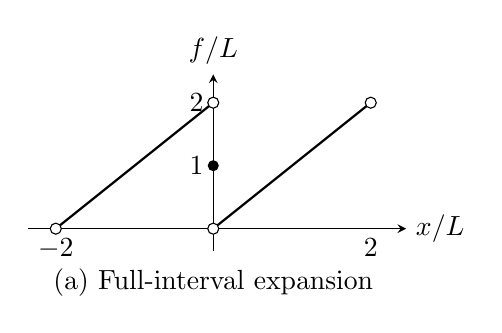
\begin{tikzpicture}[x=1cm,y=.8cm,>=stealth]
\draw[->] (-2.35,0)--(2.45,0) node[right] {$x/L$};
\draw[->] (0,-.35)--(0,2.45) node[above] {$f/L$};
\draw[thick] (-2,0)--(0,2); \draw[thick] (0,0)--(2,2);
\foreach \x/\y in {-2/0,0/2,0/0,2/2}
  \draw[fill=white] (\x,\y) circle (2pt);
\fill (0,1) circle (2pt);
\node[below] at (-2,0) {$-2$};\node[below] at (2,0) {$2$};
\node[left] at (0,1) {$1$};\node[left] at (0,2) {$2$};
\node at (0,-.85) {(a) Full-interval expansion};
\end{tikzpicture}\hspace{.6cm}
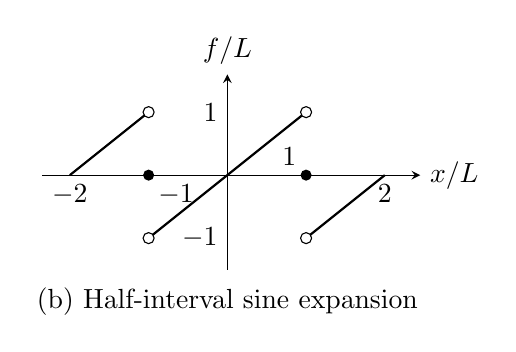
\begin{tikzpicture}[x=1cm,y=.8cm,>=stealth]
\draw[->] (-2.35,0)--(2.45,0) node[right] {$x/L$};
\draw[->] (0,-1.5)--(0,1.6) node[above] {$f/L$};
\draw[thick] (-2,0)--(-1,1);\draw[thick] (-1,-1)--(1,1);
\draw[thick] (1,-1)--(2,0);
\foreach \x/\y in {-1/1,-1/-1,1/1,1/-1}
  \draw[fill=white] (\x,\y) circle (2pt);
\fill (-1,0) circle (2pt);\fill (1,0) circle (2pt);
\node[below] at (-2,0) {$-2$};\node[below right] at (-1,0) {$-1$};
\node[above left] at (1,0) {$1$};\node[below] at (2,0) {$2$};
\node[left] at (0,1) {$1$};\node[left] at (0,-1) {$-1$};
\node at (0,-2) {(b) Half-interval sine expansion};
\end{tikzpicture}
\end{center}
Open circles are one-sided limits, and filled circles give the series
values at the indicated jumps.

\Needspace{5\baselineskip}
\par\bigskip
\noindent\textbf{19.1.10}\quad In some problems it is convenient to
approximate $\sin\pi x$ over the interval $[0,1]$ by a parabola
$ax(1-x)$, where $a$ is a constant. To get a feeling for the
accuracy of this approximation, expand $4x(1-x)$ in a Fourier sine
series ($-1\le x\le1$):
\[
f(x)=\begin{cases}
4x(1-x), & 0\le x\le1\\
4x(1+x), & -1\le x\le0
\end{cases}
=\sum_{n=1}^{\infty}b_{n}\sin n\pi x.
\]
\par\nobreak\hfill\emph{ANS.}\enspace
$b_{n}=\dfrac{32}{\pi^{3}n^{3}}$,\quad $n$ odd,\qquad
$b_{n}=0$,\quad $n$ even.
\par This approximation is shown in Fig.~19.6.
\solution
The stated extension is odd, since $f(-x)=4(-x)(1-x)=-f(x)$ for
$0\le x\le1$, so all cosine coefficients vanish. The period is $2$
($L=1$), and the integrand $f(x)\sin n\pi x$, a product of two odd
functions, is even. Put $k=n\pi$; the sine coefficient is
\[
b_n=\int_{-1}^1f(x)\sin kx\,dx=2\int_0^14x(1-x)\sin kx\,dx=8I_n,
\qquad I_n=\int_0^1x(1-x)\sin kx\,dx.
\]
Integrate by parts twice. The boundary terms vanish because
$x(1-x)=0$ at $x=0,1$ and $\sin k=\sin0=0$:
\begin{align*}
I_n&=\left[-\frac{x(1-x)\cos kx}{k}\right]_0^1
 +\frac1k\int_0^1(1-2x)\cos kx\,dx\\
&=\frac1k\left[\frac{(1-2x)\sin kx}{k}\right]_0^1
 +\frac2{k^2}\int_0^1\sin kx\,dx
 =\frac2{k^2}\,\frac{1-\cos k}{k}
 =\frac{2(1-\cos k)}{k^3}.
\end{align*}
With $\cos k=\cos n\pi=(-1)^n$ and $k^3=\pi^3n^3$, it follows that
\[
\boxed{b_n=\frac{16[1-(-1)^n]}{\pi^3n^3}
=\begin{cases}32/(\pi^3n^3),&n\text{ odd},\\0,&n\text{ even}.
\end{cases}}
\]
Thus the fundamental sine has coefficient $32/\pi^3\approx1.032$, and
the next nonzero coefficient, $b_3=32/(27\pi^3)\approx0.038$, is smaller
by a factor $27$. The series converges
absolutely and uniformly, since its terms are bounded by
$32/(\pi^3n^3)$ and $\sum n^{-3}$ converges (Weierstrass M-test). It
equals the continuous odd periodic
extension, including its zero values at $-1,0,1$.

\Needspace{5\baselineskip}
\par\bigskip
\noindent\textbf{19.1.11}\quad Verify that
$\delta(\varphi_{1}-\varphi_{2})=\dfrac{1}{2\pi}
\displaystyle\sum_{m=-\infty}^{\infty}e^{im(\varphi_{1}-\varphi_{2})}$
is a Dirac delta function by showing that it satisfies the
definition,
\[
\int_{-\pi}^{\pi}f(\varphi_{1})\,\frac{1}{2\pi}
\sum_{m=-\infty}^{\infty}e^{im(\varphi_{1}-\varphi_{2})}\,d\varphi_{1}
=f(\varphi_{2}).
\]
\par\emph{Hint.}~Represent $f(\varphi_{1})$ by an exponential
Fourier series.
\erratum{Use the periodic delta distribution on the circle, with a smooth $2\pi$-periodic test function $f$; interpret the series as the limit $N\to\infty$ of its symmetric partial sums $\sum_{m=-N}^{N}$.}
\solution
\erratum{This is the periodic delta distribution on the circle, not a
pointwise convergent series of functions: the terms $e^{imu}$ do not
tend to zero, so the series diverges at every $u$. On the real line it
is the comb $\delta_{2\pi}(u)=\sum_{k\in\mathbb Z}\delta(u-2\pi k)$.
The interval endpoints are identified.}
Take a smooth $2\pi$-periodic test function
$f(\varphi)=\sum_{j\in\mathbb Z}c_je^{ij\varphi}$, with
$c_j=(2\pi)^{-1}\int_{-\pi}^{\pi}f(\varphi)e^{-ij\varphi}\,d\varphi$.
For $j\ne0$, integrating by parts twice, with boundary terms that cancel
by periodicity, gives
\[
c_j=\frac1{2\pi ij}\int_{-\pi}^{\pi}f'(\varphi)e^{-ij\varphi}\,d\varphi
=-\frac1{2\pi j^2}\int_{-\pi}^{\pi}f''(\varphi)e^{-ij\varphi}\,d\varphi,
\]
so $|c_j|\le j^{-2}(2\pi)^{-1}\int|f''|$ and the coefficient series is
absolutely summable. For a finite symmetric kernel, interchange the
finite sum with the integral and use
$(2\pi)^{-1}\int_{-\pi}^{\pi}f(\varphi_1)e^{im\varphi_1}\,d\varphi_1=c_{-m}$:
\begin{align*}
\int_{-\pi}^{\pi}f(\varphi_1)\frac1{2\pi}
 \sum_{m=-N}^Ne^{im(\varphi_1-\varphi_2)}\,d\varphi_1
&=\sum_{m=-N}^Nc_{-m}e^{-im\varphi_2}\\
&=\sum_{j=-N}^Nc_je^{ij\varphi_2}\qquad(j=-m).
\end{align*}
The last expression is the symmetric partial sum of the Fourier series
of $f$, which converges to $f(\varphi_2)$ as $N\to\infty$ because $f$ is
smooth (Section 19.1); the absolutely summable coefficients make the
convergence uniform. This is exactly the defining distributional action,
hence
\[
\boxed{\delta_{2\pi}(\varphi_1-\varphi_2)
=\frac1{2\pi}\sum_{m\in\mathbb Z}e^{im(\varphi_1-\varphi_2)}.}
\]
For $\varphi_2$ strictly inside the integration interval, only one member
of the delta comb is present. For a piecewise regular function with a
jump at $\varphi_2$, symmetric Fourier sums give its midpoint value;
one must not assert recovery of an arbitrary assigned value at the jump.

\Needspace{5\baselineskip}
\par\bigskip
\noindent\textbf{19.1.12}\quad Show that integration of the Fourier
expansion of $f(x)=x$, $-\pi<x<\pi$, leads to
\[
\frac{\pi^{2}}{12}=\sum_{n=1}^{\infty}\frac{(-1)^{n+1}}{n^{2}}
=1-\frac{1}{4}+\frac{1}{9}-\frac{1}{16}+\cdots.
\]
\par\emph{Note.}~The series for $f(x)=x$ was the subject of
Example~19.1.1. Confirm that the change in the defined range from
$[0,2\pi]$ to $[-\pi,\pi]$ has no effect on the expansion.
\solution
From 19.1.6, or from the Fourier coefficients computed in 19.2.7,
\[
x=2\sum_{n=1}^{\infty}\frac{(-1)^{n+1}}n\sin nx,
\qquad-\pi<x<\pi.
\]
Integrating from $0$ to $x$ term by term, with
$\int_0^x\sin nt\,dt=(1-\cos nx)/n$, gives
\[
\frac{x^2}{2}
=2\sum_{n=1}^{\infty}\frac{(-1)^{n+1}}{n^2}(1-\cos nx).
\]
The integrated series is absolutely and uniformly convergent (its terms
are bounded by $4/n^2$). Termwise integration is justified as follows.
The partial sums $s_N$ of the series for $f(x)=x$ are its Fourier
partial sums, and since the trigonometric functions form a complete set,
the Fourier series of a square-integrable function converges to it in
the mean: $\|f-s_N\|_2\to0$, where
$\|g\|_2=\bigl(\int_{-\pi}^{\pi}|g|^2\,dx\bigr)^{1/2}$. By Cauchy--Schwarz
on the interval between $0$ and $x$,
\[
\Bigl|\int_0^x(f-s_N)\,dt\Bigr|\le\sqrt{|x|}\,\|f-s_N\|_2
\le\sqrt{\pi}\,\|f-s_N\|_2\longrightarrow0
\]
uniformly in $x$, so the integrated partial sums converge to
$\int_0^xt\,dt=x^2/2$.
Average the integrated identity over $(-\pi,\pi)$; uniform convergence
allows averaging term by term. Every cosine has zero average, so the
right side averages to $2\sum_{n\ge1}(-1)^{n+1}/n^2$, while
\[
\frac1{2\pi}\int_{-\pi}^{\pi}\frac{x^2}{2}\,dx
=\frac1{2\pi}\left[\frac{x^3}{6}\right]_{-\pi}^{\pi}
=\frac1{2\pi}\,\frac{2\pi^3}{6}=\frac{\pi^2}{6}.
\]
Consequently $2\sum_{n\ge1}(-1)^{n+1}/n^2=\pi^2/6$, that is,
\[
\boxed{\sum_{n=1}^{\infty}\frac{(-1)^{n+1}}{n^2}=\frac{\pi^2}{12}.}
\]
The change of range in the note does not change the underlying periodic
function: Example 19.1.1 defines it as $x$ on $(0,\pi)$ and $x-2\pi$ on
$(\pi,2\pi)$. Moving that latter interval left by $2\pi$ gives $x$ on
$(-\pi,0)$. Since the integral of a $2\pi$-periodic function is the same
over every interval of length $2\pi$, integrals over $[0,2\pi]$ and over
$[-\pi,\pi]$ give exactly these same Fourier coefficients.

\Needspace{5\baselineskip}
\par\bigskip
\noindent\textbf{19.1.13}
\begin{enumerate}
\item[(a)] Assuming that the Fourier expansion of \erratum{a real-valued} $f(x)$ is
uniformly convergent, show that
\[
\frac{1}{\pi}\int_{-\pi}^{\pi}\big[f(x)\big]^{2}dx
=\frac{a_{0}^{2}}{2}+\sum_{n=1}^{\infty}\big(a_{n}^{2}+b_{n}^{2}\big).
\]
This is Parseval's identity. Note that it is a completeness
relation for the Fourier expansion.
\item[(b)] Given
$x^{2}=\dfrac{\pi^{2}}{3}+4\displaystyle\sum_{n=1}^{\infty}
\dfrac{(-1)^{n}\cos nx}{n^{2}}$, $-\pi\le x\le\pi$, apply
Parseval's identity to obtain $\zeta(4)$ in closed form.
\item[(c)] The condition of uniform convergence is not necessary.
Show this by applying the Parseval identity to the square wave
\[
f(x)=\begin{cases}-1,&-\pi<x<0\\1,&0<x<\pi\end{cases}
=\frac{4}{\pi}\sum_{n=1}^{\infty}\frac{\sin(2n-1)x}{2n-1}.
\]
\end{enumerate}
\solution
\textbf{(a)} Square the partial sum
$s_N=a_0/2+\sum_{n=1}^N(a_n\cos nx+b_n\sin nx)$ and integrate over
$(-\pi,\pi)$. All cross terms integrate to zero, while
$\int(a_0/2)^2dx=\pi a_0^2/2$ and
$\int\cos^2nx\,dx=\int\sin^2nx\,dx=\pi$. Hence for every finite partial
sum
\[
\frac1\pi\int_{-\pi}^{\pi}s_N^2\,dx
=\frac{a_0^2}{2}+\sum_{n=1}^N(a_n^2+b_n^2).
\]
If $s_N\to f$ uniformly, that is, $\|s_N-f\|_\infty\to0$ with
$\|g\|_\infty=\sup_{-\pi<x<\pi}|g(x)|$, then $f$ is bounded, the $s_N$
are uniformly bounded for large $N$ ($\|s_N\|_\infty\le\|f\|_\infty+1$
once $\|s_N-f\|_\infty\le1$), and, since $s_N^2-f^2=(s_N-f)(s_N+f)$,
\[
\left|\int(s_N^2-f^2)\right|
\le2\pi\|s_N-f\|_\infty(\|s_N\|_\infty+\|f\|_\infty)\longrightarrow0.
\]
Letting $N\to\infty$ on both sides of the finite identity proves the
stated identity.
\erratum{The displayed identity is for real functions; the complex
version uses modulus squares. Also the Instructor's Manual's first
display in 19.1.13(a) is missing the factor $1/\pi$ on its integral:
for $f=1$ its unnormalized left side is $2\pi$, whereas its right side
is $2$.}
More generally $L^2$ convergence suffices: with $\|\cdot\|_2$ as in
19.1.12, the triangle inequality gives
$|\|s_N\|_2-\|f\|_2|\le\|s_N-f\|_2\to0$, so
$\pi^{-1}\int_{-\pi}^{\pi}s_N^2\,dx=\|s_N\|_2^2/\pi\to\|f\|_2^2/\pi$.

\textbf{(b)} Reading off the given series for $f=x^2$:
$a_0/2=\pi^2/3$, so $a_0=2\pi^2/3$; $a_n=4(-1)^n/n^2$, so
$a_n^2=16/n^4$; and $b_n=0$. The identity becomes
\[
\frac1\pi\int_{-\pi}^{\pi}x^4\,dx
=\frac1\pi\,\frac{2\pi^5}5
=\frac{2\pi^4}{5}
=\frac12\left(\frac{2\pi^2}{3}\right)^2
 +16\sum_{n=1}^{\infty}\frac1{n^4}
=\frac{2\pi^4}9+16\,\zeta(4).
\]
Solving, with $2/5-2/9=8/45$,
\[
\boxed{\zeta(4)=\frac1{16}\left(\frac25-\frac29\right)\pi^4
=\frac1{16}\,\frac{8\pi^4}{45}=\frac{\pi^4}{90}.}
\]
The given $x^2$ series is uniformly convergent by comparison with
$\sum n^{-2}$, so part (a) applies directly.

\textbf{(c)} The square wave has $f^2=1$, so
$\pi^{-1}\int_{-\pi}^{\pi}f^2\,dx=2$. From the given series it has no
constant or cosine terms, $b_{2j-1}=4/[\pi(2j-1)]$, and the even-$n$
sine coefficients vanish. Hence Parseval reads
\[
2=\frac{16}{\pi^2}\sum_{j=1}^{\infty}\frac1{(2j-1)^2}.
\]
To check this independently, the $L^2$ convergence of the square-wave
series may not be used: by the expansion in 19.1.4,
$\int(f-s_N)^2\,dx=\int f^2\,dx-\pi\sum_{n\le N}b_n^2$, so for this $f$
it is equivalent to the identity being checked. Instead use the
primitive $\int_0^xf\,dt=|x|$, which is continuous and piecewise smooth;
its cosine series (19.2.9) converges to it at every point, and at $x=0$
it gives
\[
0=\frac\pi2-\frac4\pi\sum_{j=1}^{\infty}\frac1{(2j-1)^2}.
\]
Thus $\sum_{j\ge1}(2j-1)^{-2}=\pi^2/8$ (as also found in 19.2.13(b)),
and the right side of Parseval is indeed $(16/\pi^2)(\pi^2/8)=2$.

For any fixed partial sum $s_N$, which is continuous with $s_N(0)=0$,
$s_N(x)\to0$ as $x\downarrow0$, whereas the square wave equals one there. Thus
$\sup_{0<x<\pi}|s_N(x)-1|\ge1$, ruling out uniform convergence. This supplies the requested counterexample
to necessity of uniform convergence, while $L^2$ completeness still
justifies Parseval.

\Needspace{5\baselineskip}
\par\bigskip
\noindent\textbf{19.1.14}\quad Given
\[
\varphi_{1}(x)\equiv\sum_{n=1}^{\infty}\frac{\sin nx}{n}
=\begin{cases}
-\dfrac{1}{2}(\pi+x), & -\pi\le x<0,\\[10pt]
\dfrac{1}{2}(\pi-x), & 0<x\le\pi,
\end{cases}
\]
show by integrating that
\[
\varphi_{2}(x)\equiv\sum_{n=1}^{\infty}\frac{\cos nx}{n^{2}}
=\begin{cases}
\dfrac{1}{4}(\pi+x)^{2}-\dfrac{\pi^{2}}{12}, & -\pi\le x\le0,\\[12pt]
\dfrac{1}{4}(\pi-x)^{2}-\dfrac{\pi^{2}}{12}, & 0\le x\le\pi.
\end{cases}
\]
\solution
The cosine series for $\varphi_2$ is absolutely and uniformly convergent
by comparison with $\sum n^{-2}$.
Integrating the sine series for $\varphi_1$ term by term from $0$ to $x$,
$0<x\le\pi$, is valid because the series is the Fourier series of
$\varphi_1$ (its coefficients $b_n=1/n$ are computed in 19.2.8). Its
partial sums $s_N$ therefore converge to $\varphi_1$ in the mean,
$\|\varphi_1-s_N\|_2\to0$, as in 19.1.12, and by Cauchy--Schwarz on
$(0,x)$,
\[
\Bigl|\int_0^x(\varphi_1-s_N)\,dt\Bigr|\le\sqrt{x}\,\|\varphi_1-s_N\|_2
\le\sqrt{\pi}\,\|\varphi_1-s_N\|_2\longrightarrow0.
\]
Since $n^{-1}\int_0^x\sin nt\,dt=(1-\cos nx)/n^2$, the term-by-term
integral is $\sum_{n\ge1}(1-\cos nx)/n^2=\varphi_2(0)-\varphi_2(x)$, and
integrating the closed form instead gives
\[
\varphi_2(0)-\varphi_2(x)
=\int_0^x\frac{\pi-t}{2}\,dt
=\frac{\pi x}{2}-\frac{x^2}{4}.
\]
Write $C=\varphi_2(0)$, so $\varphi_2(x)=C-\pi x/2+x^2/4$ on $[0,\pi]$.
The cosine series is even in $x$, which gives, on $[-\pi,\pi]$,
$\varphi_2(x)=C-\pi|x|/2+x^2/4$.
Every term of the uniformly convergent cosine series has zero integral
over $[0,\pi]$, because $\int_0^\pi\cos nx\,dx=\sin(n\pi)/n=0$, so
termwise integration gives
\[
0=\int_0^\pi\varphi_2(x)\,dx
=C\pi-\frac\pi2\frac{\pi^2}{2}+\frac14\frac{\pi^3}{3}
=C\pi-\frac{\pi^3}{4}+\frac{\pi^3}{12}
=C\pi-\frac{\pi^3}{6}.
\]
Therefore $C=\pi^2/6$. Completing the square,
$\pi^2/6-\pi|x|/2+x^2/4=(\pi-|x|)^2/4-\pi^2/4+\pi^2/6$, yields
\[
\boxed{\varphi_2(x)=\frac{(\pi-|x|)^2}{4}-\frac{\pi^2}{12},
\qquad -\pi\le x\le\pi,}
\]
which gives exactly the two requested branches ($|x|=-x$ for $x\le0$ and
$|x|=x$ for $x\ge0$). The derivation covered every $0\le x\le\pi$, and
evenness every $-\pi\le x\le0$, so the endpoints $x=0,\pm\pi$ are
included; in particular setting $x=0$ proves
$\sum n^{-2}=\varphi_2(0)=\pi^2/6$.

\Needspace{5\baselineskip}
\par\bigskip
\noindent\textbf{19.1.15}\quad Given
\[
\psi_{2s}(x)=\sum_{n=1}^{\infty}\frac{\sin nx}{n^{2s}},\qquad
\psi_{2s+1}(x)=\sum_{n=1}^{\infty}\frac{\cos nx}{n^{2s+1}},
\]
develop the following recurrence relations:
\begin{enumerate}
\item[(a)] $\psi_{2s}(x)=\displaystyle\int_{0}^{x}
\erratum{\psi_{2s-1}(t)\,dt}$,
\item[(b)] $\psi_{2s+1}(x)=\zeta(2s+1)
-\displaystyle\int_{0}^{x}\erratum{\psi_{2s}(t)\,dt}$.
\end{enumerate}
\par\emph{Note.}~The functions $\psi_{s}(x)$ and $\varphi_{s}(x)$
of this and the preceding exercise are known as \emph{Clausen
functions}. In theory they may be used to improve the rate of
convergence of a Fourier series. As is often the case, there is the
question of how much analytical work we do and how much arithmetic
work we demand that a computer do. As computers become steadily
more powerful, the balance progressively shifts so that we are
doing less and demanding that computers do more.
\erratum{Here $s=1,2,\ldots$. When $s=1$, the first integral is improper at multiples of $2\pi$ crossed by the interval.}
\solution
Let $s$ be a positive integer, as the statement requires: for $s=0$,
(b) would contain the divergent $\zeta(1)=\sum_n1/n$, and (a) the
divergent series $\psi_{-1}=\sum_nn\cos nx$. The statement writes the
integration variable as $t$, since $x$ is already the upper limit.
For $s\ge2$, the terms of the series for $\psi_{2s-1}$ are bounded by
$n^{-(2s-1)}\le n^{-3}$, so it converges absolutely and uniformly
(Weierstrass M-test) and may be integrated term by term, with
$\int_0^x\cos nt\,dt=\sin nx/n$. Thus
\[
\int_0^x\psi_{2s-1}(t)\,dt
=\sum_{n=1}^{\infty}\frac1{n^{2s-1}}\int_0^x\cos nt\,dt
=\sum_{n=1}^{\infty}\frac{\sin nx}{n^{2s}}
=\boxed{\psi_{2s}(x)}.
\]
For every $s\ge1$, the even-index series has terms bounded by
$n^{-2s}\le n^{-2}$, so it too converges absolutely and uniformly.
Termwise integration with $\int_0^x\sin nt\,dt=(1-\cos nx)/n$, and
splitting into two absolutely convergent series ($2s+1\ge3$), gives
\begin{align*}
\int_0^x\psi_{2s}(t)\,dt
&=\sum_{n=1}^{\infty}\frac{1-\cos nx}{n^{2s+1}}
=\sum_{n=1}^{\infty}\frac1{n^{2s+1}}
-\sum_{n=1}^{\infty}\frac{\cos nx}{n^{2s+1}}\\
&=\zeta(2s+1)-\psi_{2s+1}(x).
\end{align*}
Solving for $\psi_{2s+1}(x)$ proves the second recurrence.

\erratum{The first recurrence at $s=1$ has an integrable logarithmic
singularity at its lower endpoint: $\psi_1(t)=-\ln(2|\sin(t/2)|)$.
The integral must be read as improper at every multiple of $2\pi$ it
crosses; $\psi_1$ itself is not finite at those points.}
To justify this base case, insert $r^n$ with $0<r<1$. Then
$\sum_{n\ge1}r^n\cos nt/n=\operatorname{Re}\{-\log(1-re^{it})\}
=-\ln|1-re^{it}|$, and this series is uniformly convergent (its terms
are bounded by $r^n$), so termwise integration gives
\[
\int_0^x-\ln|1-re^{it}|\,dt
=\sum_{n=1}^{\infty}\frac{r^n\sin nx}{n^2}.
\]
The right side tends uniformly to $\psi_2(x)$ as $r\uparrow1$, because
the difference is bounded by $\sum_n(1-r^n)/n^2$, whose terms tend to
zero and are dominated by $n^{-2}$. On the left, for $t\notin2\pi\mathbb Z$
the integrand tends to $-\ln|1-e^{it}|=-\ln(2|\sin(t/2)|)=\psi_1(t)$.
To dominate it, use
\[
|1-re^{it}|^2=1-2r\cos t+r^2=(1-r)^2+4r\sin^2(t/2).
\]
For $1/2\le r<1$ this gives $2\sin^2(t/2)\le|1-re^{it}|^2<4$ (for the
lower bound drop $(1-r)^2\ge0$ and use $4r\ge2$; for the upper bound use
$|1-re^{it}|\le1+r<2$). Taking half the logarithm,
\[
\tfrac12\ln2+\ln|\sin(t/2)|\le\ln|1-re^{it}|<\ln2,
\]
and since $\ln|\sin(t/2)|\le0$ this gives
$|\ln|1-re^{it}||\le\ln2+|\ln|\sin(t/2)||$, independently of $r$. Let
$d=\operatorname{dist}(t,2\pi\mathbb Z)\in[0,\pi]$, so that
$|\sin(t/2)|=\sin(d/2)$. By Jordan's inequality ($\sin u\ge2u/\pi$ on
$[0,\pi/2]$), $\sin(d/2)\ge d/\pi$, hence
$|\ln|\sin(t/2)||\le\ln\pi-\ln d\le\ln\pi+|\ln d|$. So on any bounded
interval the integrand is bounded by $\ln(2\pi)+|\ln d|$, which is
integrable near the finitely many singularities because
$\int_0^\epsilon|\ln t|\,dt=\epsilon(1-\ln\epsilon)$ for $0<\epsilon<1$.
Dominated convergence therefore lets $r\uparrow1$ under the integral,
which proves the first recurrence also for $s=1$.

\Needspace{5\baselineskip}
\par\bigskip
\noindent\textbf{19.1.16}\quad Show that
$f(x)=\displaystyle\sum_{n=1}^{\infty}\dfrac{\cos nx}{n+1}$ may be
written as
\[
f(x)=\psi_{1}(x)-\varphi_{2}(x)
+\sum_{n=1}^{\infty}\frac{\cos nx}{n^{2}(n+1)},
\]
where $\psi_{1}(x)$ and $\varphi_{2}(x)$ are the Clausen functions
defined in Exercises~19.1.14 and 19.1.15.
\erratum{For the finite-valued identity take $x\notin2\pi\mathbb Z$.}
\solution
The elementary coefficient identity, over the common denominator
$n^2(n+1)$, is
\[
\frac1n-\frac1{n^2}+\frac1{n^2(n+1)}
=\frac{n(n+1)-(n+1)+1}{n^2(n+1)}
=\frac{n^2}{n^2(n+1)}
=\frac1{n+1}.
\]
Multiply by $\cos nx$, sum first to a finite $N$, and then pass to the
limit; for $x\notin2\pi\mathbb Z$ each of the three series converges, so
the limit of the sum is the sum of the limits. The first series is
$\psi_1=\sum\cos nx/n$ (the case $s=0$ of $\psi_{2s+1}$ in 19.1.15),
the second is $\varphi_2=\sum\cos nx/n^2$ of 19.1.14, and the last is
absolutely convergent. Therefore
\[
\boxed{f(x)=\psi_1(x)-\varphi_2(x)
+\sum_{n=1}^{\infty}\frac{\cos nx}{n^2(n+1)}.}
\]
\erratum{This equality is an ordinary finite-valued identity only for
$x\notin2\pi\mathbb Z$. At a multiple of $2\pi$ both $f$ and $\psi_1$
diverge.}
Away from those points, Dirichlet's test proves convergence of the
original series and of $\psi_1$, as in 19.1.5. The correction series has
a simple uniform truncation bound: $|\cos nx|/(n^2(n+1))<n^{-3}$, and
$n^{-3}\le\int_{n-1}^n t^{-3}\,dt$, so
\[
\left|\sum_{n>N}\frac{\cos nx}{n^2(n+1)}\right|
\le\sum_{n>N}\frac1{n^3}\le\int_N^\infty\frac{dt}{t^3}
=\frac1{2N^2}.
\]
Thus the known closed forms of the first two terms, for $0<x<2\pi$,
\[
\psi_1(x)=-\ln\Bigl(2\sin\frac x2\Bigr),\qquad
\varphi_2(x)=\frac{(\pi-x)^2}4-\frac{\pi^2}{12},
\]
leave a rapidly convergent remainder. The first is 19.1.8(b); the second
is 19.1.14 on $(0,\pi]$, extended to $[\pi,2\pi)$ by
$\varphi_2(x)=\varphi_2(x-2\pi)=\varphi_2(2\pi-x)$ (periodicity and
evenness), which reproduces the same formula.

\Needspace{12\baselineskip}
\subsection*{19.2 Applications of Fourier Series}

\Needspace{5\baselineskip}
\par\bigskip
\noindent\textbf{19.2.1}\quad Transform the Fourier expansion of a
square wave, Eq.~(19.26), into a power series \erratum{(formally: expand
each sine in powers of $x$ and collect like powers; height $h\ne0$)}.
Show that the coefficients of $x^{1}$ form a divergent series. Repeat
for the coefficients of $x^{3}$.
\par\emph{Note.}~A power series cannot handle a discontinuity.
These infinite coefficients are the result of attempting to beat
this basic limitation on power series.
\solution
Equation (19.26) is
\[
f(x)=\frac h2+\frac{2h}{\pi}\sum_{j=0}^{\infty}
\frac{\sin((2j+1)x)}{2j+1}.
\]
For each individual term its entire Taylor expansion is
\[
\frac{\sin((2j+1)x)}{2j+1}
=x-\frac{(2j+1)^2x^3}{3!}
+\frac{(2j+1)^4x^5}{5!}-\cdots.
\]
Retain only the first $N$ harmonics before collecting powers. Each
harmonic contributes $2h/\pi$ to the coefficient of $x$, so the linear
coefficient is $2hN/\pi$. For the cubic coefficient expand
$(2j+1)^2=4j^2+4j+1$ and use
$\sum_{j=0}^{N-1}j^2=(N-1)N(2N-1)/6$,
$\sum_{j=0}^{N-1}j=N(N-1)/2$:
\begin{align*}
-\frac{2h}{6\pi}\sum_{j=0}^{N-1}(2j+1)^2
&=-\frac{h}{3\pi}
\left[4\frac{(N-1)N(2N-1)}6
+4\frac{N(N-1)}2+N\right]\\
&=-\frac{h}{3\pi}\,\frac{N(4N^2-1)}3
=-\frac{hN(4N^2-1)}{9\pi},
\end{align*}
since the bracket is
$[(4N^3-6N^2+2N)+(6N^2-6N)+3N]/3=(4N^3-N)/3$.
For nonzero $h$ neither coefficient has a finite limit as $N\to\infty$;
their magnitudes grow as $N$ and $N^3$, respectively. Formally, the coefficient of
$x^{2k+1}$ would be
\[
\frac{2h}{\pi}\frac{(-1)^k}{(2k+1)!}
\sum_{j=0}^{\infty}(2j+1)^{2k},
\]
and it diverges for every $k\ge0$, because every term of the sum is at
least $1$.
\erratum{The textbook's request to transform the Fourier series into a
power series is therefore only formal, not a valid convergent
power-series rearrangement. Interchanging the harmonic
sum and Taylor sum is precisely the invalid step.}
A convergent power series on a neighborhood of zero is continuous
there, so it cannot reproduce the jump between $0$ and $h$.
Away from jumps the square wave is locally constant and has a perfectly
valid local constant Taylor series; the obstruction concerns a single
series spanning the discontinuity.

\Needspace{5\baselineskip}
\par\bigskip
\noindent\textbf{19.2.2}\quad Derive the Fourier series expansion
of the Dirac delta function $\delta(x)$ in the interval
$-\pi<x<\pi$.
\begin{enumerate}
\item[(a)] What significance can be attached to the constant term?
\item[(b)] In what region is this representation valid?
\item[(c)] With the identity
\[
\sum_{n=1}^{N}\cos nx=\frac{\sin(Nx/2)}{\sin(x/2)}
\cos\left[\erratum{(N+1)}\frac{x}{2}\right],
\]
show that your Fourier representation of $\delta(x)$ is consistent
with Eq.~(5.27).
\end{enumerate}
\erratum{Interpret the expansion distributionally. In the finite-sum identity use the continuous limiting value where $\sin(x/2)=0$.}
\solution
Apply the coefficient formulas to the distribution on $(-\pi,\pi)$,
using the sampling rule $\int_{-\pi}^{\pi}\delta(x)g(x)\,dx=g(0)$:
\[
a_0=\frac1\pi\int\delta(x)\,dx=\frac1\pi,
\quad a_n=\frac1\pi\int\delta(x)\cos nx\,dx=\frac{\cos0}\pi=\frac1\pi,
\quad b_n=\frac{\sin0}\pi=0.
\]
Thus, with $a_0/2=1/(2\pi)$,
\[
\boxed{\delta_{2\pi}(x)=\frac1{2\pi}
+\frac1\pi\sum_{n=1}^{\infty}\cos nx.}
\]
\textbf{(a)} The constant $1/(2\pi)$ is the mean density over one
period. All other terms integrate to zero over $(-\pi,\pi)$; this term
alone ensures unit total mass, $\int_{-\pi}^{\pi}dx/(2\pi)=1$.

\textbf{(b)} \erratum{The equality is distributional, and its global
extension is periodic: $\delta_{2\pi}(x)=\sum_{k\in\mathbb Z}
\delta(x-2\pi k)$. It represents the single $\delta(x)$ within
$(-\pi,\pi)$, not a single isolated delta on the whole real line.}
The series cannot be interpreted as an ordinary pointwise function.

\textbf{(c)} \erratum{The textbook's finite-sum identity has an
incorrect angle: its cosine must be $\cos((N+1)x/2)$, not
$\cos((N+1/2)x/2)$, as the geometric sum below shows.}
Indeed, factoring $e^{iNx/2}$ from the numerator and $e^{ix/2}$ from
the denominator, and using $e^{-iu}-e^{iu}=-2i\sin u$, the geometric
sum is
\begin{align*}
\sum_{n=1}^Ne^{inx}
&=e^{ix}\frac{1-e^{iNx}}{1-e^{ix}}
=e^{ix}\,\frac{e^{iNx/2}(e^{-iNx/2}-e^{iNx/2})}
{e^{ix/2}(e^{-ix/2}-e^{ix/2})}\\
&=e^{i(N+1)x/2}\frac{\sin(Nx/2)}{\sin(x/2)}.
\end{align*}
Taking real parts proves the corrected identity. Add the constant
term and use $2\sin A\cos B=\sin(A+B)+\sin(A-B)$ with $A=Nx/2$,
$B=(N+1)x/2$, so that $A+B=(N+1/2)x$ and $A-B=-x/2$. This yields
\begin{align*}
1+2\sum_{n=1}^N\cos nx
&=\frac{\sin(x/2)+\sin((N+1/2)x)-\sin(x/2)}{\sin(x/2)}\\
&=\frac{\sin((N+1/2)x)}{\sin(x/2)}=D_N(x).
\end{align*}
The quotient has the removable value $D_N(0)=2N+1$ (the left side at
$x=0$, or the limit $(N+1/2)/(1/2)$ of the quotient).
Its normalized integral is one,
$(2\pi)^{-1}\int_{-\pi}^{\pi}D_N\,dx=1$, since each $\cos nx$
integrates to zero. Moreover, since
$D_N(x)=\sum_{n=-N}^Ne^{inx}$, for a periodic $f$ with exponential
Fourier coefficients $c_n$ (as in 19.1.11)
\[
\frac1{2\pi}\int_{-\pi}^{\pi}f(x)D_N(x)\,dx=\sum_{n=-N}^Nc_{-n}
=\sum_{n=-N}^Nc_n,
\]
the symmetric partial sum of the Fourier series of $f$ at $x=0$; in
particular $D_N/(2\pi)$ reproduces the value at $0$ of every Fourier
polynomial of degree at most $N$. For smooth periodic $f$ these
partial sums tend to $f(0)$ as $N\to\infty$, as shown in 19.1.11.
This is the delta limit.

Specifically Eq. (5.27) is the closure relation
$\delta(x-t)=\sum_j\phi_j(x)\phi_j^*(t)$.
For the orthonormal functions
$1/\sqrt{2\pi}$, $\cos nx/\sqrt\pi$, $\sin nx/\sqrt\pi$,
setting $t=0$ gives
$1/(2\pi)+\pi^{-1}\sum_{n\ge1}(\cos nx\cos0+\sin nx\sin0)$,
exactly the boxed formula. Thus the finite kernel
and the general bilinear closure relation agree.

\Needspace{5\baselineskip}
\par\bigskip
\noindent\textbf{19.2.3}\quad Expand $\delta(x-t)$ in a Fourier
series. Compare your result with the bilinear form of Eq.~(5.27).
\par\nobreak\hfill\emph{ANS.}\enspace
$\delta(x-t)=\dfrac{1}{2\pi}+\dfrac{1}{\pi}
\displaystyle\sum_{n=1}^{\infty}(\cos nx\cos nt+\sin nx\sin nt)$\par
\nobreak\hfill$\hspace{4em}=\dfrac{1}{2\pi}+\dfrac{1}{\pi}
\displaystyle\sum_{n=1}^{\infty}\cos n(x-t)$.
\erratum{Use the periodic distribution on $(-\pi,\pi)$, with $t$ in that interval, or equivalently work on the circle.}
\solution
For $t$ strictly inside $(-\pi,\pi)$, the delta's sampling rule
$\int_{-\pi}^{\pi}\delta(x-t)g(x)\,dx=g(t)$, applied to $g=1$,
$\cos nx$, $\sin nx$ in the coefficient formulas, gives
\[
a_0(t)=\frac1\pi,\qquad
 a_n(t)=\frac{\cos nt}{\pi},\qquad
 b_n(t)=\frac{\sin nt}{\pi}.
\]
Substitution into $a_0/2+\sum_{n\ge1}(a_n\cos nx+b_n\sin nx)$ gives
\begin{align*}
\delta_{2\pi}(x-t)
&=\frac1{2\pi}+\frac1\pi\sum_{n=1}^{\infty}
(\cos nx\cos nt+\sin nx\sin nt)\\
&=\boxed{\frac1{2\pi}+\frac1\pi\sum_{n=1}^{\infty}\cos n(x-t)}.
\end{align*}
The last equality is the cosine subtraction identity
$\cos nx\cos nt+\sin nx\sin nt=\cos n(x-t)$, applied first to finite
sums. With the real orthonormal basis $1/\sqrt{2\pi}$,
$\cos nx/\sqrt\pi$, $\sin nx/\sqrt\pi$ from 19.2.2, the first line is
precisely $\sum_j\phi_j(x)\phi_j^*(t)$ in Eq.~(5.27), because
$(1/\sqrt{2\pi})(1/\sqrt{2\pi})=1/(2\pi)$ and
$(\cos nx/\sqrt\pi)(\cos nt/\sqrt\pi)=\pi^{-1}\cos nx\cos nt$, and
similarly for the sines.
For example, integrating against $\phi_k(x)$ leaves, by orthonormality,
only the $k$th term and gives $\phi_k(t)$; by the convergent Fourier
expansion this extends to smooth test functions.
The periodic/distributional and endpoint qualifications of 19.2.2
apply equally to the translated kernel.

\Needspace{5\baselineskip}
\par\bigskip
\noindent\textbf{19.2.4}\quad Show that integrating the Fourier
expansion of the Dirac delta function (Exercise~19.2.2) leads to
the Fourier representation of the square wave, Eq.~(19.26), with
$h=1$.
\par\emph{Note.}~Integrating the constant term $(1/2\pi)$ leads to
a term $x/2\pi$. What are you going to do with this?
\solution
Let $H(x)$ be zero for $-\pi<x<0$ and one for $0<x<\pi$.
Within this open interval, $H'=\delta(x)$ and the symmetric value at
zero is $H(0)=1/2$. Integrate the delta Fourier series from zero term
by term,
\[
\int_0^x\Bigl[\frac1{2\pi}+\frac1\pi\sum_{n=1}^{\infty}\cos nt\Bigr]dt
=\frac x{2\pi}+\frac1\pi\sum_{n=1}^{\infty}\frac{\sin nx}n,
\]
and add $H(0)=1/2$. This gives
\[
H(x)=\frac12+\frac{x}{2\pi}
+\frac1\pi\sum_{n=1}^{\infty}\frac{\sin nx}{n},
\qquad -\pi<x<\pi.
\]
As a check, by 19.1.5 the sine series is $(\pi-x)/2$ on $(0,\pi)$ and
$-(\pi+x)/2$ on $(-\pi,0)$, so the right side is
$1/2+x/(2\pi)+(\pi-x)/(2\pi)=1$ and
$1/2+x/(2\pi)-(\pi+x)/(2\pi)=0$, respectively.
The term $x/(2\pi)$ of the note must be retained; the answer to the
note's question is to replace it by its own Fourier series, the
sawtooth series $x=2\sum_{n\ge1}(-1)^{n+1}\sin nx/n$ of 19.2.7, that
is, $x/(2\pi)=\pi^{-1}\sum_{n\ge1}(-1)^{n+1}\sin nx/n$:
\begin{align*}
H(x)&=\frac12+\frac1\pi\sum_{n=1}^{\infty}
\frac{1+(-1)^{n+1}}n\sin nx\\
&=\boxed{\frac12+\frac2\pi\sum_{j=0}^{\infty}
\frac{\sin((2j+1)x)}{2j+1}}.
\end{align*}
Since $1+(-1)^{n+1}$ is $0$ for even $n$ and $2$ for odd $n=2j+1$, the
even terms cancel and the odd terms double, which is Eq.~(19.26) with
$h=1$.

There is also a direct way to keep the periodic boundary bookkeeping.
Integrate the series of 19.2.3 over $0<t<\pi$. The constant term gives
$\pi/(2\pi)=1/2$, and with $u=x-t$,
$\int_0^\pi\cos n(x-t)\,dt=\int_{x-\pi}^x\cos nu\,du
=[\sin nx-\sin(n(x-\pi))]/n$, and
$\sin(n(x-\pi))=(-1)^n\sin nx$:
\begin{align*}
H(x)&=\int_0^\pi\delta_{2\pi}(x-t)\,dt\\
&=\frac12+\frac1\pi\sum_{n=1}^{\infty}
\frac{\sin nx-\sin(n(x-\pi))}{n}\\
&=\frac12+\frac1\pi\sum_{n=1}^{\infty}
\frac{1-(-1)^n}{n}\sin nx.
\end{align*}
For $0<x<\pi$ the delta at $t=x$ lies in $(0,\pi)$ and the integral is
$1$; for $-\pi<x<0$ the comb members at $t=x$ and $t=x+2\pi$ both lie
outside $(0,\pi)$ and it is $0$. The coefficient $1-(-1)^n$ again keeps
only odd $n$, with value $2$, reproducing the boxed series.
\erratum{The Instructor's Manual's final negative-$x$ branch is
printed as $1$; it must be $0$. Also the derivative of the periodic step is
$\delta_{2\pi}(x)-\delta_{2\pi}(x-\pi)$, including the downward
boundary jump. Integrating a single periodic delta produces the linear
term above, not by itself a periodic primitive.}
At all jump points the Fourier series takes the midpoint $1/2$.

\Needspace{5\baselineskip}
\par\bigskip
\noindent\textbf{19.2.5}\quad Starting from the Fourier series
given as lines 4 and 5 of Table~19.1, show that:
\[
\sum_{n=0}^{\infty}\frac{\cos(2n+1)x}{2n+1}
=\frac{1}{2}\ln\left|\cot\frac{x}{2}\right|.
\]
\erratum{Exclude $x\in\pi\mathbb Z$.}
\solution
On $0<|x|<\pi$, the two logarithmic series in Table 19.1 read as
follows; they are 19.1.8(b), extended to $-\pi<x<0$ because both sides
are even, and 19.1.8(a) multiplied by $-1$:
\[
A(x)=\sum_{n=1}^{\infty}\frac{\cos nx}{n}
=-\ln(2|\sin(x/2)|),
\qquad
B(x)=\sum_{n=1}^{\infty}\frac{(-1)^n\cos nx}{n}
=-\ln(2\cos(x/2)).
\]
\erratum{In the Instructor's Manual's intermediate first sum, the
denominator printed as $x$ must be $n$, and that sum starts at $n=1$.}
Subtracting the two convergent series term by term eliminates every even
harmonic, since $1-(-1)^n$ is $0$ for even $n$ and $2$ for odd $n$:
\[
A-B=\sum_{n=1}^{\infty}\frac{1-(-1)^n}{n}\cos nx
=2\sum_{j=0}^{\infty}\frac{\cos((2j+1)x)}{2j+1}.
\]
The corresponding logarithmic difference is, since $\cos(x/2)>0$ for
$|x|<\pi$,
\[
\ln(2\cos(x/2))-\ln(2|\sin(x/2)|)
=\ln\frac{\cos(x/2)}{|\sin(x/2)|}
=\ln|\cot(x/2)|.
\]
Dividing $A-B$ by $2$ gives
\[
\boxed{\sum_{j=0}^{\infty}\frac{\cos((2j+1)x)}{2j+1}
=\frac12\ln|\cot(x/2)|.}
\]
\erratum{Exclude $x\in\pi\mathbb Z$. At even multiples of $\pi$
the series diverges to $+\infty$; at odd multiples it diverges to
$-\infty$.}
Elsewhere its ordinary convergence follows from Dirichlet's test for
$\sum e^{i(2j+1)x}$, whose geometric ratio is $e^{2ix}\ne1$.
Both sides have period $2\pi$, so periodicity extends the displayed
identity to every other real $x\notin\pi\mathbb Z$.

\Needspace{5\baselineskip}
\par\bigskip
\noindent\textbf{19.2.6}\quad Develop the Fourier series
representation of
\[
f(t)=\begin{cases}
0, & -\pi\le\omega t\le0,\\
\sin\omega t, & 0\le\omega t\le\pi.
\end{cases}
\]
This is the output of a simple half-wave rectifier. It is also an
approximation of the solar thermal effect that produces ``tides''
in the atmosphere.
\par\nobreak\hfill\emph{ANS.}\enspace
$f(t)=\dfrac{1}{\pi}+\dfrac{1}{2}\sin\omega t
-\dfrac{2}{\pi}\displaystyle\sum_{n=2,4,6,\ldots}
\dfrac{\cos n\omega t}{n^{2}-1}$.
\solution
Put $x=\omega t$ and use the $2\pi$-periodic extension. Only the
positive half-period contributes, so
\[
a_0=\frac1\pi\int_0^\pi\sin x\,dx=\frac2\pi.
\]
Orthogonality of sines on $(0,\pi)$ gives
\[
b_n=\frac1\pi\int_0^\pi\sin x\sin nx\,dx
=\frac1{2\pi}\int_0^\pi[\cos((n-1)x)-\cos((n+1)x)]\,dx
=\frac12\delta_{n1},
\]
because for $n\ge2$ both cosines integrate to zero, while for $n=1$ the
integrand is $1-\cos2x$, with integral $\pi$.
For $n\ne1$, the product-to-sum identity
$\sin x\cos nx=\frac12[\sin((n+1)x)+\sin((1-n)x)]$ and
$\int_0^\pi\sin mx\,dx=[1-(-1)^m]/m$ ($m\ne0$) give
\begin{align*}
a_n&=\frac1{2\pi}\int_0^\pi
 [\sin((n+1)x)+\sin((1-n)x)]\,dx\\
&=\frac1{2\pi}\left[
\frac{1-(-1)^{n+1}}{n+1}
+\frac{1-(-1)^{1-n}}{1-n}\right].
\end{align*}
For odd $n>1$ both $n+1$ and $1-n$ are even, so both numerators vanish.
For even $n$ both are odd and both numerators equal $2$, so
\[
a_n=\frac1\pi\left(\frac1{n+1}+\frac1{1-n}\right)
=\frac1\pi\,\frac{(1-n)+(n+1)}{(n+1)(1-n)}
=-\frac{2}{\pi(n^2-1)}.
\]
The exceptional coefficient is also zero:
$a_1=(2\pi)^{-1}\int_0^\pi\sin2x\,dx=0$.
Consequently, with $a_0/2=1/\pi$ and $n=2j$, $n^2-1=4j^2-1$,
\[
\boxed{f(t)=\frac1\pi+\frac12\sin\omega t
-\frac2\pi\sum_{j=1}^{\infty}
\frac{\cos(2j\omega t)}{4j^2-1}.}
\]
The coefficients of the infinite remainder are $O(j^{-2})$, so the
series converges absolutely and uniformly, including the joining points
where the rectified waveform is continuous and zero.

\Needspace{5\baselineskip}
\par\bigskip
\noindent\textbf{19.2.7}\quad A sawtooth wave is given by
\[
f(x)=x,\qquad-\pi<x<\pi.
\]
Show that
\[
f(x)=2\sum_{n=1}^{\infty}\frac{(-1)^{n+1}}{n}\sin nx.
\]
\solution
Oddness gives $a_0=a_n=0$, since $x$ and $x\cos nx$ are odd. The
integrand $x\sin nx$ is even, so with the antiderivative of 19.1.9,
$\sin n\pi=0$ and $\cos n\pi=(-1)^n$, the sine coefficient is
\begin{align*}
b_n&=\frac1\pi\int_{-\pi}^\pi x\sin nx\,dx
=\frac2\pi\int_0^\pi x\sin nx\,dx\\
&=\frac2\pi\left[-\frac{x\cos nx}{n}
+\frac{\sin nx}{n^2}\right]_0^\pi
=\frac2\pi\left(-\frac{\pi(-1)^n}{n}\right)
=\frac{2(-1)^{n+1}}n.
\end{align*}
Thus
\[
\boxed{x=2\sum_{n=1}^{\infty}\frac{(-1)^{n+1}}n\sin nx,
\qquad -\pi<x<\pi.}
\]
The periodic extension is piecewise smooth; its Fourier sum agrees
with $x$ at every point of this open interval. At $x=\pm\pi$ the
periodic extension jumps from $\pi$ to $-\pi$, and every sine term
vanishes, giving the midpoint zero.

\Needspace{5\baselineskip}
\par\bigskip
\noindent\textbf{19.2.8}\quad A different sawtooth wave is
described by
\[
f(x)=\begin{cases}
-\dfrac{1}{2}(\pi+x), & -\pi\le x<0,\\[10pt]
+\dfrac{1}{2}(\pi-x), & 0<x\le\pi.
\end{cases}
\]
Show that $f(x)=\displaystyle\sum_{n=1}^{\infty}(\sin nx/n)$.
\solution
The function is odd, so only sine terms remain. For $n\ge1$, using
$\int_0^\pi\sin nx\,dx=[1-(-1)^n]/n$ and
$\int_0^\pi x\sin nx\,dx=-\pi(-1)^n/n$ from 19.2.7,
\begin{align*}
b_n&=\frac2\pi\int_0^\pi\frac{\pi-x}{2}\sin nx\,dx\\
&=\int_0^\pi\sin nx\,dx
-\frac1\pi\int_0^\pi x\sin nx\,dx\\
&=\frac{1-(-1)^n}{n}
-\frac1\pi\left(-\frac{\pi(-1)^n}{n}\right)
=\frac{1-(-1)^n+(-1)^n}{n}=\frac1n.
\end{align*}
\erratum{The Instructor's Manual's last integral in its coefficient
calculation prints $x\sin x$; it must be $x\sin nx$. The
$n$-dependence is retained above.}
Therefore
\[
\boxed{f(x)=\sum_{n=1}^{\infty}\frac{\sin nx}{n}}
\]
throughout the stated intervals. At zero the two limiting values are
$\pm\pi/2$, and the Fourier value is zero. At $\pm\pi$ the function
and the series are both zero. This coefficient calculation independently
confirms the logarithmic summation in 19.1.5.

\Needspace{5\baselineskip}
\par\bigskip
\noindent\textbf{19.2.9}\quad A triangular wave (Fig.~19.4) is
represented by
\[
f(x)=\begin{cases}
x, & 0<x<\pi\\
-x, & -\pi<x<0.
\end{cases}
\]
Represent $f(x)$ by a Fourier series.
\par\nobreak\hfill\emph{ANS.}\enspace
$f(x)=\dfrac{\pi}{2}-\dfrac{4}{\pi}
\displaystyle\sum_{n=1,3,5,\ldots}\dfrac{\cos nx}{n^{2}}$.
\solution
Here $f(x)=|x|$ is even, so $b_n=0$ and the cosine integrals may be
taken over $(0,\pi)$ and doubled. Its constant coefficient is
\[
a_0=\frac2\pi\int_0^\pi x\,dx=\frac2\pi\,\frac{\pi^2}2=\pi.
\]
For $n\ge1$, integration by parts (the antiderivative of 19.1.9, with
$\sin n\pi=0$, $\cos n\pi=(-1)^n$) gives
\begin{align*}
a_n&=\frac2\pi\int_0^\pi x\cos nx\,dx\\
&=\frac2\pi\left[\frac{x\sin nx}{n}
+\frac{\cos nx}{n^2}\right]_0^\pi
=\frac{2[(-1)^n-1]}{\pi n^2}.
\end{align*}
Thus the even coefficients vanish, while each odd one is $-4/(\pi n^2)$;
with $a_0/2=\pi/2$,
\[
\boxed{|x|=\frac\pi2-\frac4\pi\sum_{j=0}^{\infty}
\frac{\cos((2j+1)x)}{(2j+1)^2},\qquad-\pi\le x\le\pi.}
\]
The periodic triangular wave is continuous, including at the period
endpoints, and piecewise smooth, so by Dirichlet's theorem its Fourier
series converges to it at every point; the corners at $x=0$ and
$x=\pm\pi$, where the slope jumps between $-1$ and $+1$, do not obstruct
equality. The series converges absolutely and uniformly by comparison
with $\sum n^{-2}$.

\Needspace{5\baselineskip}
\par\bigskip
\noindent\textbf{19.2.10}\quad Expand
\[
f(x)=\begin{cases}
1, & x^{2}<x_{0}^{2}\\
0, & x^{2}>x_{0}^{2}
\end{cases}
\]
in the interval $[-\pi,\pi]$.
\par\emph{Note.}~This variable-width square wave is of some
importance in electronic music.
\erratum{Take $x_0$ real and include zero width and full width; at a jump, state the Fourier midpoint value.}
\solution
Because the definition involves $x_0^2$, write $\alpha=|x_0|$.
First assume $0<\alpha<\pi$. The waveform depends only on $x^2$, so it is
even, giving $b_n=0$; on $(0,\pi)$ it is $1$ for $x<\alpha$ and $0$ for
$x>\alpha$. Hence
\[
a_0=\frac2\pi\int_0^\alpha1\,dx=\frac{2\alpha}{\pi},
\qquad
a_n=\frac2\pi\int_0^\alpha\cos nx\,dx
=\frac2\pi\left[\frac{\sin nx}n\right]_0^\alpha
=\frac{2\sin n\alpha}{n\pi},
\]
and, with $a_0/2=\alpha/\pi$,
\[
\boxed{f(x)=\frac\alpha\pi+\frac2\pi\sum_{n=1}^{\infty}
\frac{\sin n\alpha}{n}\cos nx.}
\]
The constant term is the duty fraction: the pulse occupies length
$2\alpha$ of a period $2\pi$. The series is one or zero in the open
constant regions. At the two jumps $x=\pm\alpha$ its value is the
midpoint $1/2$: with $2\sin n\alpha\cos n\alpha=\sin2n\alpha$ and
19.1.5 for $0<2\alpha<2\pi$,
\[
\frac\alpha\pi+\frac1\pi\sum_{n=1}^{\infty}\frac{\sin2n\alpha}{n}
=\frac\alpha\pi+\frac1\pi\,\frac{\pi-2\alpha}2=\frac12.
\]

\erratum{The usual variable-width formula presumes $0<|x_0|<\pi$.
For $|x_0|\ge\pi$ the function is one almost everywhere in the interval;
for $x_0=0$ it is zero almost everywhere.}
The equality points $x^2=x_0^2$ in the piecewise definition can be
assigned arbitrarily without changing any coefficient. One formula for
all real $x_0$ is obtained by replacing $\alpha$ by $\min(|x_0|,\pi)$
above: it reduces to the appropriate constant series in the two limiting
cases, since $\alpha=\pi$ gives $\alpha/\pi=1$ and $\sin n\pi=0$, and
$\alpha=0$ makes every term zero.

\Needspace{5\baselineskip}
\par\bigskip
\noindent\textbf{19.2.11}\quad A metal cylindrical tube of radius
$a$ is split lengthwise into two nontouching halves. The top half
is maintained at a potential $+V$, the bottom half at a potential
$-V$. See Fig.~19.9. Separate the variables in Laplace's equation
and solve for the electrostatic potential for $r\le a$. Observe
the resemblance between your solution for $r=a$ and the Fourier
series for a square wave.
\erratum{Assume an infinitely long tube, negligible slit width and no axial variation. Impose the boundary values away from the two ideal slit lines.}
\solution
\erratum{Use the ideal infinitely long tube, with translational symmetry
along its axis and negligible slit width. Finite end effects or a finite
open gap require additional boundary data. At the ideal slit endpoints
the two assigned boundary limits disagree, so a single boundary value
cannot be imposed there.}
Take $0<\varphi<\pi$ to be the top half. With no dependence on the axial
coordinate, Laplace's equation in the interior, in polar coordinates, is
\[
\Phi_{rr}+\frac1r\Phi_r+\frac1{r^2}\Phi_{\varphi\varphi}=0.
\]
With $\Phi=R(r)\Theta(\varphi)$, multiplication by $r^2/(R\Theta)$
separates this into a function of $r$ equal to a function of $\varphi$,
hence to a constant, written $n^2$:
\[
\frac{r^2R''+rR'}R=-\frac{\Theta''}\Theta=n^2.
\]
The angular equation $\Theta''+n^2\Theta=0$ has $2\pi$-periodic
(single-valued) solutions only for integer $n\ge0$, namely
$\Theta=\cos n\varphi,\sin n\varphi$ (for $n=0$ the general solution
$A+B\varphi$ changes by $2\pi B$ around the axis, so periodicity forces
$B=0$ and leaves the constant); a negative constant would give
nonperiodic exponentials. The radial equation $r^2R''+rR'-n^2R=0$ is
of Euler type: $R=r^k$ gives $k^2=n^2$, so $R=r^n,r^{-n}$ for $n\ge1$,
while for $n=0$ it reads $(rR')'=0$, with solutions $R=1,\ln r$.
Boundedness at the axis excludes $r^{-n}$ and $\ln r$, leaving
\[
\Phi(r,\varphi)=C_0+\sum_{n=1}^{\infty}
(r/a)^n(C_n\cos n\varphi+D_n\sin n\varphi).
\]
At $r=a$ this must be the Fourier series of the boundary function,
$V$ on $(0,\pi)$ and $-V$ on $(-\pi,0)$. That function is odd and has
zero mean, so $C_0=C_n=0$. Its sine coefficients, with the even
integrand reduced to $(0,\pi)$ and
$\int_0^\pi\sin n\varphi\,d\varphi=[1-(-1)^n]/n$, are
\[
D_n=\frac1\pi\int_{-\pi}^{\pi}\Phi(a,\varphi)\sin n\varphi\,d\varphi
=\frac2\pi\int_0^\pi V\sin n\varphi\,d\varphi
=\frac{2V}{n\pi}[1-(-1)^n],
\]
that is, $4V/(n\pi)$ for odd $n$ and $0$ for even $n$. Therefore
\[
\boxed{\Phi(r,\varphi)=\frac{4V}{\pi}\sum_{j=0}^{\infty}
\frac{(r/a)^{2j+1}}{2j+1}\sin((2j+1)\varphi),\qquad r<a.}
\]
The series and all differentiated series converge uniformly on compact
subdisks, so it is harmonic. As $r\uparrow a$, it becomes the $\pm V$
square-wave series and attains the prescribed values away from the slits.
Its radial limit on a slit is the midpoint zero.

For an additional closed-form check put $q=r/a<1$ and $z=qe^{i\varphi}$,
so that the boxed series is
$(4V/\pi)\operatorname{Im}\sum_{j\ge0}z^{2j+1}/(2j+1)$. Integrate the
geometric series $\sum_{j\ge0}z^{2j}=1/(1-z^2)$ from $0$ to $z$, using
the partial fractions $1/(1-z^2)=\frac12[1/(1+z)+1/(1-z)]$:
\[
\sum_{j=0}^{\infty}\frac{z^{2j+1}}{2j+1}
=\frac12\bigl[\log(1+z)-\log(1-z)\bigr]
=\frac12\log\frac{1+z}{1-z},
\]
with principal logarithms; $1\pm z$ lie in the right half-plane, so
their arguments lie in $(-\pi/2,\pi/2)$ and subtract without a $2\pi$
correction. Multiplying numerator and denominator by $1-\bar z$, and
using $z-\bar z=2iq\sin\varphi$,
\[
\frac{1+z}{1-z}=\frac{(1+z)(1-\bar z)}{|1-z|^2}
=\frac{1-q^2+2iq\sin\varphi}{|1-z|^2},
\]
whose real part is positive. Thus
\[
\Phi=\frac{2V}\pi\operatorname{Arg}\frac{1+z}{1-z}
=\frac{2V}\pi\arctan\frac{2q\sin\varphi}{1-q^2},
\]
and multiplying numerator and denominator by $a^2$ gives
\[
\boxed{\Phi(r,\varphi)=\frac{2V}{\pi}
\arctan\frac{2ar\sin\varphi}{a^2-r^2},\qquad r<a.}
\]
As $r\uparrow a$ the argument of the arctangent tends to $+\infty$ where
$\sin\varphi>0$ and to $-\infty$ where $\sin\varphi<0$, so the limit is
$+V$ above and $-V$ below. The bounded harmonic Dirichlet
solution is unique: the difference of two such solutions has zero
boundary data almost everywhere and its Poisson representation is zero.

\Needspace{5\baselineskip}
\par\bigskip
\noindent\textbf{19.2.12}\quad A metal cylinder is placed in a
(previously) uniform electric field, $\mathbf{E}_{0}$, with the
axis of the cylinder perpendicular to that of the original field.
\begin{enumerate}
\item[(a)] Find the perturbed electrostatic potential.
\item[(b)] Find the induced surface charge on the cylinder as a
function of angular position.
\end{enumerate}
\erratum{Assume an infinitely long neutral cylinder in vacuum. Take its radius to be $a$ and set its constant potential to zero.}
\solution
\erratum{The usual solution assumes an infinitely long, neutral cylinder
in vacuum. The textbook's problem does not specify a net charge; allowing
one adds a logarithmic monopole potential. Finite cylinders require end
data.}
Let the radius be $a$ and take the original field to be $E_0\hat{\mathbf x}$.
Choose the conductor potential as zero, so the far-field potential is
$-E_0r\cos\varphi$.

\textbf{(a)} The separated exterior harmonic functions are those of
19.2.11, $1,\ln r,r^{\pm n}\cos n\varphi,r^{\pm n}\sin n\varphi$, now
keeping $r^{-n}$ and $\ln r$ because the axis is excluded. Thus
\[
\Phi_{\rm out}=A_0+B_0\ln r+\sum_{n=1}^{\infty}
\bigl[(A_nr^n+B_nr^{-n})\cos n\varphi
+(A_n'r^n+B_n'r^{-n})\sin n\varphi\bigr].
\]
The applied field has only the $n=1$ cosine component. Since the
perturbation $\Phi_{\rm out}+E_0r\cos\varphi$ decays at infinity,
$A_1=-E_0$, every other $A_n$ and every $A_n'$ vanish, and
$A_0=B_0=0$ ($\ln r$ grows; it is the potential of a net line charge).
The conductor condition $\Phi_{\rm out}(a,\varphi)=0$ for all $\varphi$
makes every Fourier coefficient of the boundary values vanish:
$B_na^{-n}=0$ for $n\ge2$, $B_n'a^{-n}=0$ for $n\ge1$, and
$-E_0a+B_1/a=0$, or $B_1=E_0a^2$. Hence
\[
\boxed{\Phi_{\rm out}(r,\varphi)
=-E_0\left(r-\frac{a^2}{r}\right)\cos\varphi\quad(r\ge a),
\qquad\Phi_{\rm in}=0.}
\]
Each radial term solves the separated Laplace equation, and
$\Phi_{\rm out}+E_0r\cos\varphi=E_0a^2\cos\varphi/r\to0$.

\textbf{(b)} Since $\partial_r(r-a^2/r)=1+a^2/r^2$, the outward normal
field just outside the surface is
\[
E_r=-\partial_r\Phi_{\rm out}
=E_0\left(1+\frac{a^2}{r^2}\right)\cos\varphi,
\qquad E_r(a^+)=2E_0\cos\varphi.
\]
Since the field inside the metal is zero, the boundary condition
(Gauss's law for a thin pillbox across the surface) gives
\[
\boxed{\sigma(\varphi)=\epsilon_0[E_r(a^+)-E_r(a^-)]
=2\epsilon_0E_0\cos\varphi.}
\]
Also
$E_\varphi=-r^{-1}\partial_\varphi\Phi_{\rm out}
=-E_0(1-a^2/r^2)\sin\varphi$ vanishes at $r=a$, as it must on a
conductor, and the total induced charge per unit length is
$a\int_0^{2\pi}\sigma\,d\varphi=2\epsilon_0E_0a\int_0^{2\pi}\cos\varphi
\,d\varphi=0$, verifying neutrality.
If a net line charge $\lambda$ is specified instead, the more general
solution contains
\[
\Phi_{\rm mono}=-\frac{\lambda}{2\pi\epsilon_0}\ln(r/a),
\qquad \sigma_{\rm mono}=\frac{\lambda}{2\pi a},
\]
plus an arbitrary common potential constant. The decaying-perturbation
condition used above excludes this monopole.

\Needspace{5\baselineskip}
\par\bigskip
\noindent\textbf{19.2.13}
\begin{enumerate}
\item[(a)] Find the Fourier series representation of
\[
f(x)=\begin{cases}
0, & -\pi<x\le0\\
x, & 0\le x<\pi.
\end{cases}
\]
\item[(b)] From the Fourier expansion show that
\[
\frac{\pi^{2}}{8}=1+\frac{1}{3^{2}}+\frac{1}{5^{2}}+\cdots.
\]
\end{enumerate}
\solution
\textbf{(a)} Since $f=0$ on $(-\pi,0)$, all coefficient integrals run
only from zero to $\pi$:
\[
a_0=\frac1\pi\int_0^\pi x\,dx=\frac1\pi\,\frac{\pi^2}2=\frac\pi2.
\]
For $n\ge1$, the antiderivatives of $x\cos nx$ and $x\sin nx$ from
19.1.9, with $\sin n\pi=0$ and $\cos n\pi=(-1)^n$, give
\begin{align*}
a_n&=\frac1\pi\int_0^\pi x\cos nx\,dx
=\frac1\pi\left[\frac{x\sin nx}{n}
+\frac{\cos nx}{n^2}\right]_0^\pi
=\frac{(-1)^n-1}{\pi n^2},\\
b_n&=\frac1\pi\int_0^\pi x\sin nx\,dx
=\frac1\pi\left[-\frac{x\cos nx}{n}
+\frac{\sin nx}{n^2}\right]_0^\pi
=\frac{(-1)^{n+1}}n.
\end{align*}
Thus $a_0/2=\pi/4$, and $a_n=-2/(\pi n^2)$ for odd $n$ and $0$ for even
$n$:
\[
\boxed{f(x)=\frac\pi4-\frac2\pi\sum_{j=0}^{\infty}
\frac{\cos((2j+1)x)}{(2j+1)^2}
+\sum_{n=1}^{\infty}\frac{(-1)^{n+1}\sin nx}{n}.}
\]
This also follows by splitting $f(x)=(|x|+x)/2$ and taking half the sum
of the triangular expansion of 19.2.9 and the sawtooth expansion of
19.2.7. The function is piecewise smooth, so by Dirichlet's theorem the
equality holds on $(-\pi,\pi)$, including zero, where $f$ is continuous.
At the period endpoints the series equals the midpoint $\pi/2$ of the
jump between $f(\pi^-)=\pi$ and $f(-\pi^+)=0$.

\textbf{(b)} Set $x=0$, where $f(0)=0$. All sine terms vanish and every
cosine is one, so
\[
0=\frac\pi4-\frac2\pi\sum_{j=0}^{\infty}\frac1{(2j+1)^2}.
\]
Solving, $\sum_j(2j+1)^{-2}=(\pi/2)(\pi/4)$, gives
\[
\boxed{\sum_{j=0}^{\infty}\frac1{(2j+1)^2}=\frac{\pi^2}{8}.}
\]

\Needspace{5\baselineskip}
\par\bigskip
\noindent\textbf{19.2.14}\quad Integrate the Fourier expansion of
the unit step function
\[
f(x)=\begin{cases}
0, & -\pi<x<0\\
1, & 0<x<\pi.
\end{cases}
\]
Show that your integrated series agrees with Exercise~19.2.13.
\solution
The unit step has the series (Eq.~(19.26) with $h=1$; see 19.2.4)
\[
H(t)=\frac12+\frac2\pi\sum_{j=0}^{\infty}
\frac{\sin((2j+1)t)}{2j+1}.
\]
Its integral $F(x)=\int_0^xH(t)\,dt$ is $0$ for $-\pi<x<0$, where $H=0$
between $x$ and $0$, and $x$ for $0<x<\pi$; this is the function $f$
of 19.2.13. Integrating term by term, with
$\int_0^x\sin((2j+1)t)\,dt=[1-\cos((2j+1)x)]/(2j+1)$, gives
\[
F(x)=\frac x2+\frac2\pi\sum_{j=0}^{\infty}
\frac{1-\cos((2j+1)x)}{(2j+1)^2}.
\]
This step is justified in $L^2$: integration against the indicator of
$(0,x)$ is a bounded linear functional, and the Fourier partial sums
converge in $L^2$. The resulting series converges absolutely and
uniformly, since its terms are bounded by $(4/\pi)(2j+1)^{-2}$.
Splitting it into two absolutely convergent series and using
$\sum_{j\ge0}(2j+1)^{-2}=\pi^2/8$ (19.2.13(b)), so that the constant part
is $(2/\pi)(\pi^2/8)=\pi/4$, yields
\[
F(x)=\frac\pi4+\frac x2-\frac2\pi\sum_{j=0}^{\infty}
\frac{\cos((2j+1)x)}{(2j+1)^2}.
\]
Finally, on $(-\pi,\pi)$, half of the sawtooth series of 19.2.7 gives
$x/2=\sum_{n\ge1}(-1)^{n+1}\sin nx/n$. Substituting it produces
exactly the constant, cosine and sine terms in 19.2.13. The integral
$F$ itself is not periodic, because of its linear term $x/2$; replacing
that term by the sawtooth series supplies the required periodic
extension, with midpoint values at the endpoints.

\Needspace{5\baselineskip}
\par\bigskip
\noindent\textbf{19.2.15}\quad In the interval $(-\pi,\pi)$,
\[
\delta_{n}(x)=\begin{cases}
n, & |x| < 1/2n,\\
0, & |x| > 1/2n.
\end{cases}
\]
This wave form is the pulse shown in Fig.~19.10.
\begin{enumerate}
\item[(a)] Expand $\delta_{n}(x)$ as a Fourier cosine series.
\item[(b)] Show that your Fourier series agrees with a Fourier
expansion of $\delta(x)$ \erratum{in the distributional limit} as $n\to\infty$.
\end{enumerate}
\solution
Use a different letter $m$ for the Fourier harmonic. The pulse has
half-width $1/(2n)\le1/2<\pi$, so it lies inside the interval, and total
area $n(1/n)=1$. It is even, so $b_m=0$. Since $\delta_n$ vanishes for
$|x|>1/(2n)$ and $\cos mx$ is even, its coefficients are
\begin{gather*}
a_0=\frac1\pi\int_{-1/(2n)}^{1/(2n)}n\,dx=\frac1\pi,\\
a_m=\frac1\pi\int_{-1/(2n)}^{1/(2n)}n\cos mx\,dx
=\frac{2n}{\pi}\int_0^{1/(2n)}\cos mx\,dx
=\frac{2n}{\pi}\left[\frac{\sin mx}{m}\right]_0^{1/(2n)}
=\frac{2n}{\pi m}\sin\frac{m}{2n}.
\end{gather*}
\textbf{(a)} Therefore, with $a_0/2=1/(2\pi)$,
\[
\boxed{\delta_n(x)=\frac1{2\pi}
+\frac{2n}{\pi}\sum_{m=1}^{\infty}
\frac{\sin(m/(2n))}{m}\cos mx.}
\]
By Dirichlet's theorem (the pulse is piecewise constant), for each fixed
$n$ the series converges to the pulse away from its two edges, and to
the mean $(n+0)/2=n/2$ at the edges $x=\pm1/(2n)$.

\textbf{(b)} At every fixed harmonic $m$, the argument $u=m/(2n)$ tends
to zero and $\sin u/u\to1$, so
\[
\frac{2n}{m}\sin\frac{m}{2n}
=\frac{\sin(m/(2n))}{m/(2n)}\longrightarrow1,
\qquad
a_m=\frac1\pi\,\frac{\sin(m/(2n))}{m/(2n)}\longrightarrow\frac1\pi.
\]
The limiting coefficients therefore give
$1/(2\pi)+(1/\pi)\sum_{m\ge1}\cos mx$, the delta expansion of 19.2.2.
\erratum{This is a distributional limit; taking the coefficient limit
is not justification for a pointwise limit of the infinite series.}
A direct proof uses any test function $f$ continuous at zero. Since
$n\int_{-1/(2n)}^{1/(2n)}dx=1$, write $f(0)=n\int_{-1/(2n)}^{1/(2n)}f(0)\,dx$;
the remaining integral runs over an interval of length $1/n$, so
\[
\left|\int f(x)\delta_n(x)\,dx-f(0)\right|
=\left|n\int_{-1/(2n)}^{1/(2n)}[f(x)-f(0)]\,dx\right|
\le\sup_{|x|\le1/(2n)}|f(x)-f(0)|\longrightarrow0.
\]
This proves $\delta_n\to\delta$ directly, without passing to the limit
in the coefficients.

\Needspace{5\baselineskip}
\par\bigskip
\noindent\textbf{19.2.16}\quad Confirm the delta function nature of
your Fourier series of Exercise~19.2.15 by showing that for any
$f(x)$ that is \erratum{bounded and measurable} in $[-\pi,\pi]$ and continuous
at $x=0$,
\[
\erratum{\lim_{n\to\infty}\lim_{M\to\infty}
\int_{-\pi}^{\pi}f(x)S_{n,M}(x)\,dx=f(0).}
\]
\erratum{Here $S_{n,M}$ is the partial sum of the Fourier series of the finite-width pulse $\delta_n$ through the harmonic $\cos Mx$.}
\solution
\erratum{The displayed integrals require an integrable test function;
the textbook's hypothesis that $f$ be finite in $[-\pi,\pi]$ (pointwise
finiteness) does not by itself ensure integrability. A bounded
measurable $f$ continuous at zero suffices. The Fourier expansion must
first represent the finite-width pulse, followed by the pulse-width
limit; no unrestricted interchange of two infinite limits is needed.}
By 19.2.15(a), for fixed $n$ the partial sums are
\[
S_{n,M}(x)=\frac1{2\pi}+\sum_{m=1}^{M}a_m\cos mx,
\qquad a_m=\frac{2n}{\pi m}\sin\frac{m}{2n},
\]
and the full series equals $\delta_n$ except at the two edges. The
difference $\delta_n-S_{n,M}$ has the cosine coefficients $a_m$ for
$m>M$ and no others, so Parseval's identity on $(-\pi,\pi)$ and
$|a_m|\le2n/(\pi m)$ give
\[
\|\delta_n-S_{n,M}\|_2^2=\int_{-\pi}^{\pi}(\delta_n-S_{n,M})^2\,dx
=\pi\sum_{m>M}a_m^2\le\frac{4n^2}{\pi}\sum_{m>M}\frac1{m^2}
\longrightarrow0\quad(M\to\infty).
\]
Parseval's identity (19.1.13) applies here although the series of the
discontinuous $\delta_n$ does not converge uniformly: by the $L^2$
completeness of the Fourier basis, noted in 19.1.13(c), it holds for
every square-integrable function.
If $|f|\le B$, then $f\in L^2[-\pi,\pi]$ with $\|f\|_2\le B\sqrt{2\pi}$,
and the Cauchy--Schwarz inequality gives
\[
\left|\int_{-\pi}^{\pi}f\,(S_{n,M}-\delta_n)\,dx\right|
\le\|f\|_2\,\|S_{n,M}-\delta_n\|_2\longrightarrow0.
\]
Consequently the inner limit is the action of the pulse itself; with
$x=u/n$,
\[
I_n=\lim_{M\to\infty}\int_{-\pi}^{\pi}f(x)S_{n,M}(x)\,dx
=n\int_{-1/(2n)}^{1/(2n)}f(x)\,dx
=\int_{-1/2}^{1/2}f(u/n)\,du.
\]
Given $\epsilon>0$, continuity at zero provides $\eta>0$ such that
$|f(x)-f(0)|<\epsilon$ when $|x|<\eta$. Choose $n>1/(2\eta)$.
Then throughout the last integral $|u/n|\le1/(2n)<\eta$. Since the
$u$-interval has length one, $f(0)=\int_{-1/2}^{1/2}f(0)\,du$ and
\[
|I_n-f(0)|
\le\int_{-1/2}^{1/2}|f(u/n)-f(0)|\,du\le\epsilon.
\]
Hence
\[
\boxed{\lim_{n\to\infty}\lim_{M\to\infty}
\int_{-\pi}^{\pi}f(x)S_{n,M}(x)\,dx=f(0).}
\]
The shrinking-interval step uses only the values of $f$ near zero, so
$\int f\delta_n\,dx\to f(0)$ holds for every integrable $f$ continuous
at zero. The order of the limits matters: letting $n\to\infty$ first in
the coefficients would leave
$\int_{-\pi}^{\pi}f(x)\bigl[1/(2\pi)+\pi^{-1}\sum_{m=1}^M\cos mx\bigr]dx$,
which is the $M$th Fourier partial sum of $f$ at $x=0$, and that need
not converge even for a continuous $f$ (du Bois-Reymond constructed a
continuous periodic function whose Fourier series diverges at a point,
which a shift moves to $x=0$).

\Needspace{5\baselineskip}
\par\bigskip
\noindent\textbf{19.2.17}
\begin{enumerate}
\item[(a)] Show that the Dirac delta function $\delta(x-a)$,
expanded in a Fourier sine series in the half-interval $(0,L)$
($0<a<L$) is given by
\[
\delta(x-a)=\frac{2}{L}\sum_{n=1}^{\infty}
\sin\frac{n\pi a}{L}\sin\frac{n\pi x}{L}.
\]
Note that this series actually describes
$-\delta(x+a)+\delta(x-a)$ in the interval $(-L,L)$.
\item[(b)] By integrating both sides of the preceding equation
from $0$ to $x$, show that the cosine expansion of the square wave
\[
f(x)=\begin{cases}
0, & 0\le x<a\\
1, & a<x<L,
\end{cases}
\]
is
\[
f(x)=\frac{2}{\pi}\sum_{n=1}^{\infty}\frac{1}{n}
\sin\frac{n\pi a}{L}-\frac{2}{\pi}\sum_{n=1}^{\infty}\frac{1}{n}
\sin\frac{n\pi a}{L}\cos\frac{n\pi x}{L},
\]
for $0\le x<L$.
\item[(c)] Show that the term
$\dfrac{2}{\pi}\displaystyle\sum_{n=1}^{\infty}\dfrac{1}{n}
\sin\dfrac{n\pi a}{L}$ is the average of $f(x)$ on $(0,L)$.
\end{enumerate}
\erratum{The delta expansion is distributional. At $x=a$ the integrated Fourier series has the midpoint value $1/2$.}
\solution
\textbf{(a)} The sine functions are orthogonal on the half interval
$(0,L)$, with squared norm $L/2$ ($\delta_{nm}$ is the Kronecker delta):
\[
\int_0^L\sin\frac{n\pi x}{L}\sin\frac{m\pi x}{L}\,dx
=\frac L2\delta_{nm}.
\]
This follows by writing the product as half the difference of cosines,
\[
\sin\frac{n\pi x}{L}\sin\frac{m\pi x}{L}
=\frac12\Bigl[\cos\frac{(n-m)\pi x}{L}-\cos\frac{(n+m)\pi x}{L}\Bigr]:
\]
every $\cos(j\pi x/L)$ with $j\ne0$ integrates to zero over $(0,L)$, and
for $n=m$ the constant term $\frac12$ integrates to $L/2$. Multiplying
$\sum_nb_n\sin(n\pi x/L)$ by $\sin(m\pi x/L)$ and integrating over
$(0,L)$ therefore isolates
$(L/2)b_m$, and the sifting property ($0<a<L$) gives the delta
coefficient
\[
b_n=\frac2L\int_0^L\delta(x-a)\sin\frac{n\pi x}{L}\,dx
=\frac2L\sin\frac{n\pi a}{L},
\]
which gives the requested expansion
\[
\boxed{\delta(x-a)=\frac2L\sum_{n=1}^{\infty}
\sin\frac{n\pi a}{L}\sin\frac{n\pi x}{L},\qquad0<x,a<L.}
\]
The equality is distributional. Each $\sin(n\pi x/L)$ is odd and has
period $2L$, so on $(-L,L)$ the series represents the odd extension
$\delta(x-a)-\delta(x+a)$, repeated with period $2L$.

\textbf{(b)} For $0\le x<L$, $x\ne a$, integrating $\delta(t-a)$ from
zero to $x$ gives the step $H(x-a)$: zero for $x<a$, one for $x>a$.
For each mode,
\[
\int_0^x\sin\frac{n\pi t}{L}\,dt
=\frac{L}{n\pi}\left(1-\cos\frac{n\pi x}{L}\right),
\]
and multiplying by the coefficient $(2/L)\sin(n\pi a/L)$ gives
$(2/(n\pi))\sin(n\pi a/L)\,[1-\cos(n\pi x/L)]$. Therefore
\[
\boxed{H(x-a)=\frac2\pi\sum_{n=1}^{\infty}
\frac{\sin(n\pi a/L)}n
-\frac2\pi\sum_{n=1}^{\infty}
\frac{\sin(n\pi a/L)}n\cos\frac{n\pi x}{L}.}
\]
The termwise integration of the delta series is formal, since that
series does not converge as a function. The result is nevertheless
exact: the boxed series is the Fourier cosine series of the step on
$(0,L)$, computed directly in 19.2.18 (its constant term is
$1-a/L$ by (c)), so by Dirichlet's theorem it converges to $H(x-a)$ for
$x\ne a$ and to the midpoint $1/2$ at the jump $x=a$. At the endpoints,
$x=0$ makes the two sums cancel, giving $0$; at $x=L$,
$\cos n\pi=(-1)^n$ leaves
\[
\frac2\pi\sum_{n=1}^{\infty}\frac{\sin(n\pi a/L)}n\,\bigl[1-(-1)^n\bigr]
=\frac4\pi\sum_{n\ \mathrm{odd}}\frac{\sin(n\pi a/L)}n=1,
\]
because the square-wave series of 19.2.4 gives
$\sum_{n\ \mathrm{odd}}\sin(n\theta)/n=\pi/4$ for $0<\theta<\pi$.

\textbf{(c)} Put $\theta=\pi a/L\in(0,\pi)$ in 19.1.5:
\[
\frac2\pi\sum_{n=1}^{\infty}\frac{\sin n\theta}{n}
=\frac2\pi\frac{\pi-\theta}{2}=1-\frac aL.
\]
Independently the step average is
$L^{-1}\int_0^Lf(x)\,dx=L^{-1}\int_a^L1\,dx=1-a/L$.
Thus the first sum is exactly the required average.

\Needspace{5\baselineskip}
\par\bigskip
\noindent\textbf{19.2.18}\quad Verify the Fourier cosine expansion
of the square wave, Exercise~19.2.17(b), by direct calculation of
the Fourier coefficients.
\solution
For a half-interval cosine expansion, write
$f(x)=a_0/2+\sum_{n\ge1}a_n\cos(n\pi x/L)$. On $(0,L)$ the functions
$1,\cos(\pi x/L),\cos(2\pi x/L),\ldots$ are orthogonal, with
$\int_0^L1\,dx=L$ and $\int_0^L\cos^2(n\pi x/L)\,dx=L/2$ for $n\ge1$.
Multiplying the expansion by $1$ or by $\cos(n\pi x/L)$ and integrating
over $(0,L)$ therefore gives
$a_n=(2/L)\int_0^Lf(x)\cos(n\pi x/L)\,dx$ for all $n\ge0$. Since $f=0$
on $(0,a)$, only $(a,L)$ contributes:
\[
a_0=\frac2L\int_a^L1\,dx=2\left(1-\frac aL\right),
\]
and, for $n\ge1$, using $\sin n\pi=0$,
\[
a_n=\frac2L\int_a^L\cos\frac{n\pi x}{L}\,dx
=\frac2{n\pi}\left[\sin\frac{n\pi x}{L}\right]_a^L
=-\frac2{n\pi}\sin\frac{n\pi a}{L}.
\]
Hence, with $a_0/2=1-a/L$,
\[
\boxed{f(x)=1-\frac aL-\frac2\pi\sum_{n=1}^{\infty}
\frac{\sin(n\pi a/L)}n\cos\frac{n\pi x}{L}.}
\]
By 19.2.17(c), $(2/\pi)\sum_n\sin(n\pi a/L)/n=1-a/L$, so the constant
terms agree and the two expansions coincide term by term. The even
extension of $f$ is periodic with period $2L$; it is continuous at
$0,L$ and jumps at $\pm a$. Thus, by Dirichlet's theorem, the series has
the specified step values away from the jumps and the midpoint $1/2$
there.

\Needspace{5\baselineskip}
\par\bigskip
\noindent\textbf{19.2.19}
\begin{enumerate}
\item[(a)] A string is clamped at both ends $x=0$ and $x=L$.
Assuming small-amplitude vibrations, we find that the amplitude
$y(x,t)$ satisfies the wave equation
\[
\frac{\partial^{2}y}{\partial x^{2}}
=\frac{1}{v^{2}}\frac{\partial^{2}y}{\partial t^{2}}.
\]
Here $v$ is the wave velocity. The string is set in vibration by a
sharp blow at $x=a$. Hence we have
\[
y(x,0)=0,\qquad\frac{\partial y(x,t)}{\partial t}
=Lv_{0}\delta(x-a)\quad\text{at }t=0.
\]
The constant $L$ is included to compensate for the dimensions
(inverse length) of $\delta(x-a)$. With $\delta(x-a)$ given by
Exercise~19.2.17(a), solve the wave equation subject to these
initial conditions.
\par\nobreak\hfill\emph{ANS.}\enspace
$y(x,t)=\dfrac{2v_{0}L}{\pi v}\displaystyle\sum_{n=1}^{\infty}
\dfrac{1}{n}\sin\dfrac{n\pi a}{L}\sin\dfrac{n\pi x}{L}
\sin\dfrac{n\pi vt}{L}$.
\item[(b)] Show that the transverse velocity of the string
$\partial y(x,t)/\partial t$ is given by
\[
\frac{\partial y(x,t)}{\partial t}
=2v_{0}\sum_{n=1}^{\infty}\sin\frac{n\pi a}{L}
\sin\frac{n\pi x}{L}\cos\frac{n\pi vt}{L}.
\]
\end{enumerate}
\erratum{Take $L,v>0$ and $0<a<L$. Interpret the impulsive initial velocity and its propagated series as distributions.}
\solution
\textbf{(a)} Put $k_n=n\pi/L$ and $\Omega_n=vk_n$.
The fixed-end condition selects the sine modes, so write
$y(x,t)=\sum_{n\ge1}q_n(t)\sin k_nx$. Since
$(\sin k_nx)''=-k_n^2\sin k_nx$, substitution into $v^2y_{xx}=y_{tt}$
gives $\sum_n(q_n''+\Omega_n^2q_n)\sin k_nx=0$. Multiplying by
$\sin k_mx$ and integrating over $(0,L)$ (sine orthogonality, as in
19.2.17(a)) isolates each mode:
\[
q_n''+\Omega_n^2q_n=0,
\qquad q_n(t)=A_n\cos\Omega_nt+B_n\sin\Omega_nt.
\]
The zero initial displacement $y(x,0)=\sum_nA_n\sin k_nx=0$ forces
$A_n=0$. The sine coefficient of the initial velocity is
\[
q_n'(0)=\frac2L\int_0^L Lv_0\delta(x-a)\sin k_nx\,dx
=2v_0\sin k_na.
\]
Since $q_n'(0)=\Omega_nB_n$,
\[
B_n=\frac{2v_0\sin k_na}{\Omega_n}
=\frac{2v_0L}{\pi v}\,\frac{\sin(n\pi a/L)}{n},
\]
and we obtain
\[
\boxed{y(x,t)=\frac{2v_0L}{\pi v}\sum_{n=1}^{\infty}
\frac{\sin(n\pi a/L)\sin(n\pi x/L)\sin(n\pi vt/L)}n.}
\]
Every mode solves the wave equation and vanishes at both fixed ends.

\textbf{(b)} Differentiating $\sin\Omega_nt$ gives
$\Omega_n\cos\Omega_nt$, and the factor $\Omega_n=n\pi v/L$ cancels the
denominator and prefactor,
$(2v_0L/(\pi v))(1/n)(n\pi v/L)=2v_0$:
\[
\boxed{y_t(x,t)=2v_0\sum_{n=1}^{\infty}
\sin\frac{n\pi a}{L}\sin\frac{n\pi x}{L}
\cos\frac{n\pi vt}{L}.}
\]
At $t=0$ the series is
$Lv_0\cdot(2/L)\sum_n\sin(n\pi a/L)\sin(n\pi x/L)$, which by the sine
closure relation of 19.2.17(a) is exactly $Lv_0\delta(x-a)$.
\erratum{The ideal impulse makes the velocity a distribution. The
last series is not asserted to converge as an ordinary velocity function;
differentiation and initial conditions are interpreted distributionally.}

For an independent propagation description, extend the initial velocity
oddly and periodically:
\[
G(s)=Lv_0\sum_{j\in\mathbb Z}
[\delta(s-a-2jL)-\delta(s+a-2jL)].
\]
With zero initial displacement, d'Alembert's formula gives
\[
y(x,t)=\frac1{2v}\int_{x-vt}^{x+vt}G(s)\,ds,
\qquad y_t(x,t)=\frac12[G(x+vt)+G(x-vt)],
\]
the second by differentiating the limits of integration. $G$ is odd
about $s=0$ and, being odd with period $2L$, also about $s=L$, so its
integrals over $(-vt,vt)$ and $(L-vt,L+vt)$ vanish: $y(0,t)=y(L,t)=0$,
and the clamps hold. For $vt<\min(a,L-a)$ and $0<x<L$, the only source
that can lie in $(x-vt,x+vt)$ is the one at $s=a$ (every other source
lies at $s\le-a$ or $s\ge2L-a$, outside the interval, because
$x-vt>-vt>-a$ and $x+vt<L+vt<2L-a$), and it does exactly
when $|x-a|<vt$. Thus, before either pulse reaches an end,
$y=Lv_0/(2v)$ where $|x-a|<vt$, and zero outside; the moving fronts and
subsequent reflected images explain the singular velocity. This
confirms the Fourier solution: the sine coefficients of this plateau are
\[
\frac2L\,\frac{Lv_0}{2v}\int_{a-vt}^{a+vt}\sin k_nx\,dx
=\frac{v_0}{vk_n}\bigl[\cos k_n(a-vt)-\cos k_n(a+vt)\bigr]
=\frac{2v_0L}{\pi v}\,\frac{\sin k_na}{n}\,\sin\Omega_nt,
\]
the last step by $\cos(A-B)-\cos(A+B)=2\sin A\sin B$ (with $A=k_na$,
$B=k_nvt=\Omega_nt$) and $1/(vk_n)=L/(n\pi v)$. These are exactly the
coefficients $B_n\sin\Omega_nt$ found in (a).

\Needspace{5\baselineskip}
\par\bigskip
\noindent\textbf{19.2.20}\quad A string, clamped at $x=0$ and at
$x=L$, is vibrating freely. Its motion is described by the wave
equation
\[
\frac{\partial^{2}u(x,t)}{\partial t^{2}}
=v^{2}\frac{\partial^{2}u(x,t)}{\partial x^{2}}.
\]
Assume a Fourier expansion of the form
\[
u(x,t)=\sum_{n=1}^{\infty}b_{n}(t)\sin\frac{n\pi x}{L}
\]
and determine the coefficients $b_{n}(t)$. The initial conditions
are
\[
u(x,0)=f(x)\qquad\text{and}\qquad
\frac{\partial}{\partial t}\,u(x,0)=g(x).
\]
\par\emph{Note.}~This is only half the conventional Fourier
orthogonality integral interval. However, as long as only the
sines are included here, the Sturm--Liouville boundary conditions
are still satisfied and the functions are orthogonal.
\par\nobreak\hfill\emph{ANS.}\enspace
$b_{n}(t)=A_{n}\cos\dfrac{n\pi vt}{L}+B_{n}\sin
\dfrac{n\pi vt}{L}$,\par\nobreak
\hfill$A_{n}=\dfrac{2}{L}\displaystyle\int_{0}^{L}
f(x)\sin\frac{n\pi x}{L}\,dx$,\quad
$B_{n}=\dfrac{2}{n\pi v}\displaystyle\int_{0}^{L}
g(x)\sin\frac{n\pi x}{L}\,dx$.
\par\smallskip
\erratum{Take $L,v>0$ and real initial data. Because the modal series is differentiated termwise, it gives a classical solution only for data smooth enough and compatible with the clamps; for $f\in H_0^1(0,L)$ and $g\in L^2(0,L)$ (finite initial energy) it gives the finite-energy solution.}
\solution
Here $H_0^1(0,L)$ means that $f$ and its weak first derivative are
square integrable and $f$ has zero endpoint values. Thus the assumptions
make the initial displacement-gradient and velocity energies finite.
Let $k_n=n\pi/L$ and $\Omega_n=vk_n$, with $L,v>0$.
Substitute the sine expansion into the wave equation:
\[
\sum_{n\ge1}[b_n''(t)+\Omega_n^2b_n(t)]\sin k_nx=0.
\]
Multiplying by $\sin k_mx$ and integrating from $0$ to $L$ isolates
$(L/2)[b_m''+\Omega_m^2b_m]=0$. Thus
\[
b_n(t)=A_n\cos\Omega_nt+B_n\sin\Omega_nt.
\]
At zero, $b_n(0)=A_n$ and $b_n'(0)=\Omega_nB_n$, so the initial
conditions read
\[
\sum_{n\ge1}A_n\sin k_nx=f(x),\qquad
\sum_{n\ge1}\Omega_nB_n\sin k_nx=g(x).
\]
Projecting each onto its sine mode (multiply by $\sin k_mx$ and
integrate over $(0,L)$) gives $(L/2)A_m=\int_0^Lf\sin k_mx\,dx$ and
$(L/2)\Omega_mB_m=\int_0^Lg\sin k_mx\,dx$, that is,
\[
\boxed{A_n=\frac2L\int_0^Lf(x)\sin\frac{n\pi x}{L}\,dx,\qquad
 B_n=\frac{2}{n\pi v}\int_0^Lg(x)\sin\frac{n\pi x}{L}\,dx.}
\]
Together with the displayed time dependence these determine the solution.
The factor $2/(n\pi v)$ is $(2/L)/\Omega_n=(2/L)\,L/(n\pi v)$. The
cosine time factor carries the initial displacement, and the sine time
factor carries the initial velocity.

\erratum{For a classical solution the initial data must be regular enough
for the differentiations and compatible with the clamps (in particular
$f(0)=f(L)=0$, and $g(0)=g(L)=0$ when these traces exist). For less regular
data the modal formula is interpreted in the corresponding weak sense.}
For example $f\in H_0^1(0,L)$ and $g\in L^2(0,L)$ give a finite-energy
solution. Since $u_t=\sum_nb_n'\sin k_nx$ and
$u_x=\sum_nk_nb_n\cos k_nx$, and the sines and the cosines are each
orthogonal on $(0,L)$ with squared norms $L/2$, we have
$\int_0^Lu_t^2\,dx=(L/2)\sum_n(b_n')^2$ and
$\int_0^Lu_x^2\,dx=(L/2)\sum_nk_n^2b_n^2$. With $v^2k_n^2=\Omega_n^2$,
the energy
\[
E(t)=\frac12\int_0^L(u_t^2+v^2u_x^2)\,dx
=\frac L4\sum_{n\ge1}[(b_n')^2+\Omega_n^2b_n^2]
\]
is constant, since each summand has derivative
$2b_n'(b_n''+\Omega_n^2b_n)=0$.

\Needspace{5\baselineskip}
\par\bigskip
\noindent\textbf{19.2.21}
\begin{enumerate}
\item[(a)] Let us continue the vibrating string problem in
Exercise~19.2.20. We assume now that the presence of a resisting
medium will damp the vibrations according to the equation
\[
\frac{\partial^{2}u(x,t)}{\partial t^{2}}
=v^{2}\frac{\partial^{2}u(x,t)}{\partial x^{2}}
-k\frac{\partial u(x,t)}{\partial t}.
\]
Introduce a Fourier expansion
\[
u(x,t)=\sum_{n=1}^{\infty}b_{n}(t)\sin\frac{n\pi x}{L}
\]
and again determine the coefficients $b_{n}(t)$. Take the initial
and boundary conditions to be the same as in Exercise~19.2.20.
Assume the damping to be small.
\erratum{Since damping is small or large only relative to each mode's
frequency $n\pi v/L$, take $k\ge0$ and first consider each mode for which
$k<2n\pi v/L$.}
\item[(b)] Repeat, but assume the damping to be large.
\erratum{That is, treat the modes with $k>2n\pi v/L$, and include the
critical case $k=2n\pi v/L$; explain why finite $k$ cannot overdamp every mode.}
\end{enumerate}
\par\nobreak\hfill\emph{ANS.}\enspace
(a) $b_{n}(t)=e^{-kt/2}\big[A_{n}\cos\omega_{n}t
+B_{n}\sin\omega_{n}t\big]$,\quad
$\omega_{n}^{2}=\erratum{\left(\dfrac{n\pi v}{L}\right)^{2}}
-\left(\dfrac{k}{2}\right)^{2}>0$,\par\nobreak
\hfill$A_{n}=\dfrac{2}{L}\displaystyle\int_{0}^{L}
f(x)\sin\frac{n\pi x}{L}\,dx$,\quad
$B_{n}=\dfrac{2}{\omega_{n}L}\displaystyle\int_{0}^{L}
g(x)\sin\frac{n\pi x}{L}\,dx+\dfrac{k}{2\omega_{n}}\,A_{n}$.\par
\nobreak\hfill
(b) $b_{n}(t)=e^{-kt/2}\big[A_{n}\cosh\sigma_{n}t
+B_{n}\sinh\sigma_{n}t\big]$,\quad
$\sigma_{n}^{2}=\left(\dfrac{k}{2}\right)^{2}
-\left(\dfrac{n\pi v}{L}\right)^{2}>0$,\par\nobreak
\hfill$A_{n}=\dfrac{2}{L}\displaystyle\int_{0}^{L}
f(x)\sin\frac{n\pi x}{L}\,dx$,\quad
$B_{n}=\dfrac{2}{\sigma_{n}L}\displaystyle\int_{0}^{L}
g(x)\sin\frac{n\pi x}{L}\,dx+\dfrac{k}{2\sigma_{n}}\,A_{n}$.
\solution
Assume $k\ge0$, write $\Omega_n=n\pi v/L$, and let the initial sine coefficients be
\[
F_n=\frac2L\int_0^Lf(x)\sin\frac{n\pi x}{L}\,dx,
\qquad G_n=\frac2L\int_0^Lg(x)\sin\frac{n\pi x}{L}\,dx.
\]
Substituting the expansion into the damped wave equation gives
$\sum_n(b_n''+kb_n'+\Omega_n^2b_n)\sin(n\pi x/L)=0$, and projecting
onto each sine mode as in 19.2.20 gives
\[
b_n''+kb_n'+\Omega_n^2b_n=0,
\qquad b_n(0)=F_n,\quad b_n'(0)=G_n.
\]
To remove the first derivative put $b_n=e^{-kt/2}z_n$.
Then
\[
b_n'=e^{-kt/2}(z_n'-kz_n/2),\quad
b_n''=e^{-kt/2}(z_n''-kz_n'+k^2z_n/4),
\]
so that
\begin{align*}
b_n''+kb_n'+\Omega_n^2b_n
&=e^{-kt/2}\Bigl[z_n''-kz_n'+\frac{k^2}{4}z_n
+kz_n'-\frac{k^2}{2}z_n+\Omega_n^2z_n\Bigr]\\
&=e^{-kt/2}\Bigl[z_n''+\Bigl(\Omega_n^2-\frac{k^2}{4}\Bigr)z_n\Bigr].
\end{align*}
At $t=0$, $z_n(0)=b_n(0)$ and, from the expression for $b_n'$,
$z_n'(0)=b_n'(0)+kb_n(0)/2$. Hence
\[
z_n''+(\Omega_n^2-k^2/4)z_n=0,
\quad z_n(0)=F_n,\quad z_n'(0)=G_n+kF_n/2.
\]
\textbf{(a) Underdamped modes.} If $\Omega_n>k/2$, define
$\omega_n=\sqrt{\Omega_n^2-k^2/4}>0$. Then
$z_n=C_n\cos\omega_nt+D_n\sin\omega_nt$, and the initial conditions
give $C_n=z_n(0)=F_n$ and $\omega_nD_n=z_n'(0)=G_n+kF_n/2$, so
\[
\boxed{b_n=e^{-kt/2}\left[F_n\cos\omega_nt
+\frac{G_n+kF_n/2}{\omega_n}\sin\omega_nt\right].}
\]
This is the printed formula with $A_n=F_n$ and
$B_n=(G_n+kA_n/2)/\omega_n$.
\erratum{The textbook's answer to (a) omits the square on $n\pi v/L$ in
$\omega_n^2$; the equation for $z_n$ shows that the correct formula is
$\omega_n^2=(n\pi v/L)^2-(k/2)^2$, as used in the answer above.}

\textbf{(b) Overdamped modes.} If $0<\Omega_n<k/2$, define
$\sigma_n=\sqrt{k^2/4-\Omega_n^2}>0$. Now
$z_n=C_n\cosh\sigma_nt+D_n\sinh\sigma_nt$ with $C_n=F_n$ and
$\sigma_nD_n=G_n+kF_n/2$, so
\[
\boxed{b_n=e^{-kt/2}\left[F_n\cosh\sigma_nt
+\frac{G_n+kF_n/2}{\sigma_n}\sinh\sigma_nt\right].}
\]
This is the printed formula with $A_n=F_n$ and
$B_n=(G_n+kA_n/2)/\sigma_n$. The two decay exponents
$-k/2\pm\sigma_n$ are negative, since $0<\sigma_n<k/2$.

\erratum{Damping is classified mode by mode. No finite $k$ overdamps
all infinitely many modes, since $\Omega_n$ grows without bound.
The critical case $\Omega_n=k/2$, omitted from the textbook's question,
also needs a separate formula.}
Here $z_n''=0$, so $z_n=F_n+(G_n+kF_n/2)t$ and
\[
\boxed{b_n=e^{-kt/2}[F_n+(G_n+kF_n/2)t].}
\]
This is also the continuous $\omega_n\to0$ or $\sigma_n\to0$ limit,
since $\sin(\omega_nt)/\omega_n\to t$, $\sinh(\sigma_nt)/\sigma_n\to t$
and the cosine and hyperbolic cosine tend to $1$.
All modes are underdamped if $k<2\pi v/L$, because then
$\Omega_n\ge\Omega_1=\pi v/L>k/2$; otherwise modes with
$n<kL/(2\pi v)$ are overdamped, equality is critical, and the larger
indices remain underdamped.
As a check, let $E=\tfrac12\int_0^L(u_t^2+v^2u_x^2)\,dx$.
Differentiating and integrating the second term by parts gives
\begin{align*}
E'&=\int_0^L(u_tu_{tt}+v^2u_xu_{xt})\,dx\\
&=v^2[u_xu_t]_0^L+\int_0^Lu_t(u_{tt}-v^2u_{xx})\,dx\\
&=-k\int_0^Lu_t^2\,dx\le0\qquad(k\ge0).
\end{align*}
The boundary term vanishes because the clamped displacement is constant
in time, hence $u_t=0$ at both ends, and the last line uses the equation
of motion, $u_{tt}-v^2u_{xx}=-ku_t$. For smooth data this is a direct
calculation; for finite-energy data it follows by limits of finite modal
sums. It is consistent with the time dependence of every mode: as in
19.2.20, $E=(L/4)\sum_n[(b_n')^2+\Omega_n^2b_n^2]$, and the mode
equation $b_n''+\Omega_n^2b_n=-kb_n'$ gives each summand the derivative
$2b_n'(b_n''+\Omega_n^2b_n)=-2k(b_n')^2$, so
$E'=-(kL/2)\sum_n(b_n')^2=-k\int_0^Lu_t^2\,dx$, as found above.

\Needspace{12\baselineskip}
\subsection*{19.3 Gibbs Phenomenon}

\Needspace{5\baselineskip}
\par\bigskip
\noindent\textbf{19.3.1}\quad With the partial-sum summation
techniques of this section, show that at a discontinuity in $f(x)$
the Fourier series for $f(x)$ takes on the arithmetic mean of the
right- and left-hand limits:
\[
\erratum{\lim_{r\to\infty}s_r(x_{0})}=\tfrac{1}{2}\big[f(x_{0}+0)+f(x_{0}-0)\big].
\]
In evaluating $\displaystyle\lim_{r\to\infty}s_{r}(x_{0})$, you may
find it convenient to identify part of the integrand as a Dirac
delta function.
\erratum{Assume $f$ is $2\pi$-periodic and of bounded variation on a period. The left side is the Fourier-series limit, regardless of the assigned value of $f(x_0)$.}
\solution
\erratum{The conclusion concerns the Fourier-series value, which need
not equal an arbitrarily assigned $f(x_0)$. As in the chapter's Dirichlet
conditions, assume a piecewise regular periodic function; bounded
variation suffices. The existence of a jump alone is not a general
pointwise-convergence hypothesis. The textbook's Eq. (19.29) also omits
$n$ from the exponential; the correct finite kernel uses $e^{in(x-t)}$,
as in Eq. (19.30).}
Write $N$ for the textbook's number $r$ of harmonics, so that $s_N$ is
its $s_r$. The variation of a function $\varphi$ on an interval $J$ is
$\operatorname{Var}_J\varphi
=\sup\sum_{i=1}^k|\varphi(t_i)-\varphi(t_{i-1})|$, the supremum over all
finite chains $t_0<t_1<\dots<t_k$ in $J$, and $f$ has bounded variation
when its variation over a period is finite. Such an $f$ is a difference
of two increasing functions (Jordan decomposition), so the one-sided
limits $f(x_0\pm0)$ exist. Let
\[
m=\frac{f(x_0+0)+f(x_0-0)}2,
\qquad D_N(t)=\frac{\sin((N+1/2)t)}{\sin(t/2)}.
\]
Inserting the coefficient integrals into
$s_N(x)=a_0/2+\sum_{n=1}^N(a_n\cos nx+b_n\sin nx)$ and using
$\cos nt\cos nx+\sin nt\sin nx=\cos n(t-x)$ gives the finite
partial-sum formula
\[
s_N(x)=\frac1{2\pi}\int_{-\pi}^{\pi}f(t)
\Bigl[1+2\sum_{n=1}^N\cos n(t-x)\Bigr]dt
=\frac1{2\pi}\int_{-\pi}^{\pi}f(t)D_N(t-x)\,dt,
\]
because the finite geometric sum is
\[
1+2\sum_{n=1}^N\cos nu=\sum_{n=-N}^{N}e^{inu}
=\frac{e^{-iNu}\bigl(e^{i(2N+1)u}-1\bigr)}{e^{iu}-1}
=\frac{e^{i(N+1/2)u}-e^{-i(N+1/2)u}}{e^{iu/2}-e^{-iu/2}}
=D_N(u).
\]
Put $t=x_0+s$; the integrand has period $2\pi$ in $s$, so $s$ may
still run over $(-\pi,\pi)$. On $(-\pi,0)$ replace $s$ by $-s$, using
that $D_N$ is even, and rename $s$ as $t$:
\[
s_N(x_0)=\frac1{2\pi}\int_0^\pi
[f(x_0+t)+f(x_0-t)]D_N(t)\,dt.
\]
Because $D_N=1+2\sum_{j=1}^N\cos jt$ and $\int_0^\pi\cos jt\,dt
=\sin j\pi/j=0$, the integral of $D_N$ on $(0,\pi)$ is exactly $\pi$,
so $m=(2\pi)^{-1}\int_0^\pi2m\,D_N(t)\,dt$. Subtracting $m$ therefore
gives
\[
s_N(x_0)-m=\frac1{2\pi}\int_0^\pi g(t)D_N(t)\,dt,
\quad g(t)=f(x_0+t)+f(x_0-t)-2m,
\quad g(0+)=0.
\]
We prove that the last integral tends to zero, including its potentially
singular neighborhood of zero.

Put $M=N+1/2$ and $A_N(u)=\int_0^uD_N(t)\,dt$ for $0\le u\le\pi$.
Split
\[
\frac1{\sin(t/2)}=\frac2t+q(t),\qquad
A_N(u)=2\int_0^{Mu}\frac{\sin v}{v}\,dv
+\int_0^u q(t)\sin Mt\,dt,
\]
the first integral by the substitution $v=Mt$.
Here $q(t)=t/12+O(t^3)$ at zero, so $q$ is continuous on $[0,\pi]$ and
integrable. The sine integral is uniformly bounded: below $v=1$,
$|\sin v/v|\le1$ makes its absolute integral at most one; beyond one,
integration by parts gives
\[
\int_1^z\frac{\sin v}{v}\,dv
=\left[-\frac{\cos v}{v}\right]_1^z
-\int_1^z\frac{\cos v}{v^2}\,dv,
\]
whose absolute value is at most
$\cos1+1/z+\int_1^zv^{-2}\,dv=1+\cos1<2$. Hence
$|\int_0^z\sin v/v\,dv|\le3$ for every $z\ge0$, and consequently
$|A_N(u)|\le C=6+\int_0^\pi|q(t)|\,dt$, independently of $N,u$.

Since $g$ has bounded variation (the variation of a sum is at most the
sum of the variations) and $g(0+)=0$, choose a small
$\delta>0$ for which both $|g(\delta)|$ and its variation on
$(0,\delta]$ are small. Since $dA_N=D_N\,dt$ and the boundary term at
zero vanishes ($A_N(0)=0$, $g(0+)=0$), Stieltjes integration by parts
gives
\[
\left|\int_0^\delta g(t)D_N(t)\,dt\right|
=\left|g(\delta)A_N(\delta)-\int_{(0,\delta]}A_N(t)\,dg(t)\right|
\le C\bigl(|g(\delta)|+\operatorname{Var}_{(0,\delta]}g\bigr).
\]
The last step uses $|A_N|\le C$: every Riemann--Stieltjes sum
$\sum_iA_N(\xi_i)[g(t_i)-g(t_{i-1})]$ of $\int A_N\,dg$ is at most
$C\sum_i|g(t_i)-g(t_{i-1})|\le C\operatorname{Var}_{(0,\delta]}g$ in
absolute value.
The variation $\operatorname{Var}_{(0,\delta]}g$ can only decrease as
$\delta\downarrow0$, and its limit is zero: if it stayed above some
$\eta>0$, we could take a chain in $(0,\pi]$ with sum above $\eta/2$,
starting at some $t_0>0$, then such a chain in $(0,t_0/2]$, and so on;
joined, $K$ of these chains form one chain in $(0,\pi]$ with sum above
$K\eta/2$, impossible for large $K$ because $g$ has bounded variation.
Also $g(\delta)\to0$. Thus the bound tends to zero as
$\delta\downarrow0$, uniformly in $N$.
For fixed $\delta$, the remaining integrand on $[\delta,\pi]$ has the
form $h(t)\sin Mt$ with $h(t)=g(t)/\sin(t/2)$, which is bounded by
$\sup|g|/\sin(\delta/2)$ and Riemann integrable (monotone functions are,
$g$ is a combination of them, and $1/\sin(t/2)$ is continuous there). Its integral
tends to zero as $M\to\infty$ by the Riemann--Lebesgue lemma: given
$\epsilon>0$, take a step function $s$ with
$\int_\delta^\pi|h-s|\,dt<\epsilon$ (a lower Darboux step function of
$h$ will do). Each of the finitely many sine integrals of $s$ is
$O(1/M)$, since $|\int_\alpha^\beta\sin Mt\,dt|\le2/M$, while
$|\int_\delta^\pi(h-s)\sin Mt\,dt|<\epsilon$ for every $M$; hence
$\limsup_{M\to\infty}|\int_\delta^\pi h(t)\sin Mt\,dt|\le\epsilon$ for
every $\epsilon>0$. Combining the two parts, for every such $\delta$
\[
\limsup_{N\to\infty}|s_N(x_0)-m|
\le\frac{C}{2\pi}\bigl(|g(\delta)|+\operatorname{Var}_{(0,\delta]}g\bigr),
\]
and the right side tends to zero as $\delta\downarrow0$. This proves
\[
\boxed{\lim_{N\to\infty}s_N(x_0)
=\frac{f(x_0+0)+f(x_0-0)}2.}
\]
This is the precise form of the hint: on $(0,\pi)$ the kernel
$D_N/(2\pi)$ has total weight $1/2$ and acts in the limit as half a
Dirac delta function at $t=0$ on $f(x_0+t)+f(x_0-t)$. The kernel's
symmetry is what assigns equal weight to the two one-sided limits.

\Needspace{5\baselineskip}
\par\bigskip
\noindent\textbf{19.3.2}\quad Determine the partial sum, $s_{n}$,
of the series in Eq.~(19.33) by using
\begin{enumerate}
\item[(a)] $\dfrac{\sin mx}{m}
=\displaystyle\int_{0}^{x}\cos my\,dy$,
\item[(b)] $\displaystyle\sum_{p=1}^{n}\cos(2p-1)y
=\dfrac{\sin 2ny}{2\sin y}$.
\end{enumerate}
\erratum{Compare the peak limit with Eqs.~(19.38) and (19.41) (the
textbook cites Eq.~(19.40) here; see the solution).}
\solution
Equation (19.33) represents levels $\pm h/2$. Its first $n$ nonzero
harmonics give
\[
s_n(x)=\frac{2h}{\pi}\sum_{p=1}^n
\frac{\sin((2p-1)x)}{2p-1}.
\]
By hint (a) with $m=2p-1$, each term is
$\sin((2p-1)x)/(2p-1)=\int_0^x\cos((2p-1)y)\,dy$. There are only
finitely many terms, so the finite sum and the integral may be
interchanged:
\[
s_n(x)=\frac{2h}{\pi}\int_0^x\sum_{p=1}^n\cos((2p-1)y)\,dy.
\]
The identity in hint (b) follows by telescoping: the product formula
$2\sin A\cos B=\sin(A+B)+\sin(A-B)$ with $A=y$, $B=(2p-1)y$ gives
\[
2\sin y\cos((2p-1)y)=\sin2py-\sin(2p-2)y,
\]
so the sum over $p=1,\ldots,n$ collapses to $\sin2ny-\sin0=\sin2ny$.
Consequently, since $(2h/\pi)/2=h/\pi$, the exact partial sum is
\[
\boxed{s_n(x)=\frac h\pi\int_0^x\frac{\sin2ny}{\sin y}\,dy.}
\]
The apparent singularities at multiples of $\pi$ are removable because
the quotient equals twice a finite cosine sum.
For $h>0$, its first positive maximum occurs at $x_n=\pi/(2n)$: by the
fundamental theorem of calculus the derivative is
$(h/\pi)\sin2nx/\sin x$, positive for $0<x<\pi/(2n)$ and negative for
$\pi/(2n)<x<\pi/n$. Changing variables $t=2ny$ ($dy=dt/(2n)$, and
$y=x_n$ becomes $t=\pi$) at that maximum gives
\[
s_n(x_n)=\frac h\pi\int_0^\pi
\frac{\sin t}{2n\sin(t/(2n))}\,dt
=\frac h\pi\int_0^\pi\frac{\sin t}{t}\,
\frac{t/(2n)}{\sin(t/(2n))}\,dt
\longrightarrow\frac h\pi\int_0^\pi\frac{\sin t}{t}\,dt.
\]
The limit holds because $u/\sin u$ increases on $(0,\pi/2)$ (its
derivative is $(\sin u-u\cos u)/\sin^2u$, and $\sin u-u\cos u$ vanishes
at $u=0$ and has derivative $u\sin u>0$), so for
$0<t\le\pi$ the last factor lies between $1$ and
$(\pi/(2n))/\sin(\pi/(2n))$, which tends to $1$; the factor therefore
tends to $1$ uniformly, and $|\sin t/t|\le1$.
More generally, at $x=z/(2n)$ for fixed $z$ the limiting profile is
$(h/\pi)\int_0^z\sin t/t\,dt$.

\erratum{Eq. (19.40), cited at the end of the textbook's question, is a
tail-integral identity, not a partial-sum formula. The exact expression
above agrees with the small-$x$ approximation in (19.37) and the peak
limit in (19.38). Using (19.40) together with
$\int_0^\infty\sin t/t\,dt=\pi/2$ gives the peak integral in (19.41).}
Thus the limiting peak is
$(h/\pi)\int_0^\pi\sin t/t\,dt=(h/2)\,(2/\pi)\int_0^\pi\sin t/t\,dt
=(h/2)I$, with $I=1.178979744\ldots$ computed in 19.3.3. Its overshoot
above the level $h/2$ is $(h/2)(I-1)\approx0.08949h$: about $8.949\%$
of the jump height $h$, or $17.898\%$ of the positive level $h/2$.

\Needspace{5\baselineskip}
\par\bigskip
\noindent\textbf{19.3.3}
\begin{enumerate}
\item[(a)] Calculate the value of the Gibbs phenomenon integral
\[
I=\frac{2}{\pi}\int_{0}^{\pi}\frac{\sin t}{t}\,dt
\]
by numerical quadrature accurate to 12 significant figures.
\item[(b)] Check your result by (1) expanding the integrand as a
series, (2) integrating term by term, and (3) evaluating the
integrated series. This calls for double-precision calculation.
\end{enumerate}
\par\nobreak\hfill\emph{ANS.}\enspace$I=1.178979744472$.
\solution
\textbf{(a)} Define the removable endpoint by $(\sin t/t)|_{t=0}=1$.
Map the $n$-point Gauss--Legendre rule to $[0,\pi]$: with $t=\pi(1+x)/2$
the prefactor $2/\pi$ cancels $dt=(\pi/2)\,dx$, so with the Legendre
nodes $x_j$ (the zeros of $P_n$) and weights
$w_j=2/[(1-x_j^2)P_n'(x_j)^2]$ on $[-1,1]$,
\[
I=\int_{-1}^{1}\frac{\sin t}{t}\,dx
\approx Q_n=\sum_{j=1}^nw_j\,\frac{\sin t_j}{t_j},
\qquad t_j=\frac\pi2(1+x_j).
\]
Because the integrand is entire, the error $Q_n-I$ falls very fast
with $n$:
it is $-2.9\times10^{-12}$ for $n=6$, $7.5\times10^{-15}$ for $n=7$,
$-1.5\times10^{-17}$ for $n=8$ and $1.3\times10^{-38}$ for $n=15$.
Thus $n=7$ in ordinary double precision already gives the requested
twelve significant figures, and $n=20$ in 65-digit arithmetic gives
\[
\boxed{I=1.178979744472167270232028845824\ldots.}
\]
Adaptive tanh--sinh quadrature at the same precision gives the same
digits. To twelve significant figures the result is
$\boxed{1.17897974447}$; the textbook's $1.178979744472$ agrees when
rounded to twelve decimal places.

\textbf{(b)} The entire power series for the integrand is
\[
\frac{\sin t}{t}=\sum_{k=0}^{\infty}
\frac{(-1)^kt^{2k}}{(2k+1)!}.
\]
On $[0,\pi]$ its terms are bounded by $\pi^{2k}/(2k+1)!$, the terms of
a convergent series, so by the Weierstrass M-test it converges
uniformly there and may be integrated termwise. With
$\int_0^\pi t^{2k}\,dt=\pi^{2k+1}/(2k+1)$,
\begin{align*}
I&=\frac2\pi\sum_{k=0}^{\infty}
\frac{(-1)^k}{(2k+1)!}\frac{\pi^{2k+1}}{2k+1}\\
&=\boxed{2\sum_{k=0}^{\infty}
\frac{(-1)^k\pi^{2k}}{(2k+1)(2k+1)!}}.
\end{align*}
Let $T_k=2\pi^{2k}/[(2k+1)(2k+1)!]$. Since
$(2k+3)!=(2k+3)(2k+2)(2k+1)!$, successive magnitudes satisfy
\[
\frac{T_{k+1}}{T_k}
=\frac{\pi^2(2k+1)\,(2k+1)!}{(2k+3)\,(2k+3)!}
=\frac{\pi^2(2k+1)}{(2k+3)^2(2k+2)}<1\qquad(k\ge0).
\]
To verify the inequality for every $k$, put
$r_k=(2k+1)/[(2k+3)^2(2k+2)]$. Over the common denominator, using
$2k+2=2(k+1)$ and $2k+4=2(k+2)$, the numerator of $r_k-r_{k+1}$ is
$(2k+1)(k+2)(2k+5)^2-(k+1)(2k+3)^3$, so
\[
r_k-r_{k+1}
=\frac{16k^3+68k^2+84k+23}
 {2(k+1)(k+2)(2k+3)^2(2k+5)^2}>0\qquad(k\ge0).
\]
Thus the ratios decrease, and the largest is $\pi^2r_0=\pi^2/18<1$.
The magnitudes $T_k$ therefore decrease monotonically to zero, and by
the alternating-series (Leibniz) test the remainder after $N$ terms is
at most $T_N$. Direct evaluation in high-precision arithmetic yields
\[
\begin{array}{r|l|l}
N&\text{sum of terms }k=0,\ldots,N-1&\text{bound }T_N\\\hline
4&1.1735737377034521530&5.811\times10^{-3}\\
8&1.1789797154459948275&2.978\times10^{-8}\\
12&1.1789797444721629210&4.406\times10^{-15}\\
16&1.1789797444721672702&5.658\times10^{-23}
\end{array}
\]
These bounds concern the mathematical series truncation; arithmetic
roundoff must be controlled separately. Summing the sixteen terms using
ordinary double-precision arithmetic and compensated summation gives
$1.178979744472167$, independently meeting the requested twelve-digit
accuracy. High-precision series evaluation and both quadrature methods
provide the additional cross-checks.
